\documentclass[a4paper,12pt]{report}
\usepackage[spanish]{babel}
\usepackage[utf8]{inputenc}
\usepackage{graphicx, csquotes, longtable, array, booktabs, xparse, float, titlesec, enumitem, dingbat, soul, multicol, listings}
\usepackage[dvipsnames]{xcolor}
\usepackage[margin=2cm]{geometry}
\usepackage{subfigure}
\usepackage{graphicx}
\setlength{\fboxsep}{0pt}
\setlength{\fboxrule}{1pt}


% Añadir la bibliografía
%\usepackage[backend=biber, style=numeric, sorting=ynt]{biblatex}
%\addbibresource{guia.bib}

% Cambia el color de los links
\usepackage{hyperref}
\hypersetup{hidelinks}

% Elimina la palabra "Capítulo" de los títulos de los capítulos
\titleformat{\chapter}[display]
  {\normalfont\bfseries}{}{0pt}{\Huge\thechapter.\space}

\titleformat{name=\chapter,numberless}[display]
  {\normalfont\bfseries}{}{0pt}{\Huge}

\titlespacing*{\chapter}{0pt}{-50pt}{20pt}

% Idioma predeterminado (Español)
\selectlanguage{spanish}

\begin{document}
  \begin{titlepage}
    \centering
    
\includegraphics[width=0.6\textwidth]{../.img/ehuLogoLargo.jpg}\\
    \vspace{1cm}
    \LARGE Aula Open Data de la UPV/EHU\\
    \vspace{0.5cm}
    \Large Ingeniería Informática de Gestión y Sistemas de Información\\
    \vspace{3cm}
    \vspace{0.5cm}
    \Huge \textbf{UNIGO}\\
    \huge ehunzango\\
    \vspace{2.5cm}
    \Large Autores:\\
    \vspace{0.2cm}
    \large Dueñas Fernandez, Iñigo\\
    \large Etxaniz Monge, Eneko\\
    \large Gabiña Barañano, Xabier\\
    \large Palacios Orueta, Irune\\
    \vfill
    \today
  \end{titlepage}
  
\chapter{Introducción}
  El proyecto \textbf{UNIGO - Aula Open Data de la UPV/EHU} consiste en el desarrollo de una aplicación móvil para el sistema operativo Android, orientada a facilitar el acceso al campus de Álava desde cualquier punto de la ciudad de Vitoria-Gasteiz. La aplicación integra múltiples modos de transporte (a pie, en bicicleta y en autobús urbano), utilizando datos abiertos provenientes de diversas fuentes oficiales, tales como el Gobierno Vasco, Euskotren y Tuvisa.
  
  La aplicación es compatible con dispositivos que usen Android 10 (API nivel 29) o superior. No se podrá instalar ni ejecutar en versiones anteriores. Al mismo tiempo, está optimizada y probada para funcionar correctamente en Android 15 (API nivel 35).
  
\chapter{Manual de uso}
\section{Acceso}
  Al abrir la aplicación por primera vez, se muestra una \textit{Splash screen} (Figura \ref{fig:splash}) donde el usuario tendrá que deslizar la pantalla hacia arriba para acceder a UNIGO. Esto llevará a una pantalla de inicio de sesión, donde el usuario podrá autenticarse su correo electrónico y contraseña (Figura \ref{fig:inicial}). También existe una pestaña de registro para introducir el nombre completo, correo electrónico y contraseña. Otras opciones incluyen continuar con Google o continuar en modo anónimo, sin cuenta. Este sistema se ha gestionado mediante Firebase, y cabe mencionar que mientras el usuario no cierre sesión, esta se mantendrá iniciada en el dispositivo para futuras ocasiones en las que entre a la aplicación: no será necesario deslizar hacia arriba en la \textit{Splash screen}, porque se realizará la autenticación automáticamente.

\vspace{0.3cm}

% splash
\begin{figure}[htbp]
  \centering
  \fbox{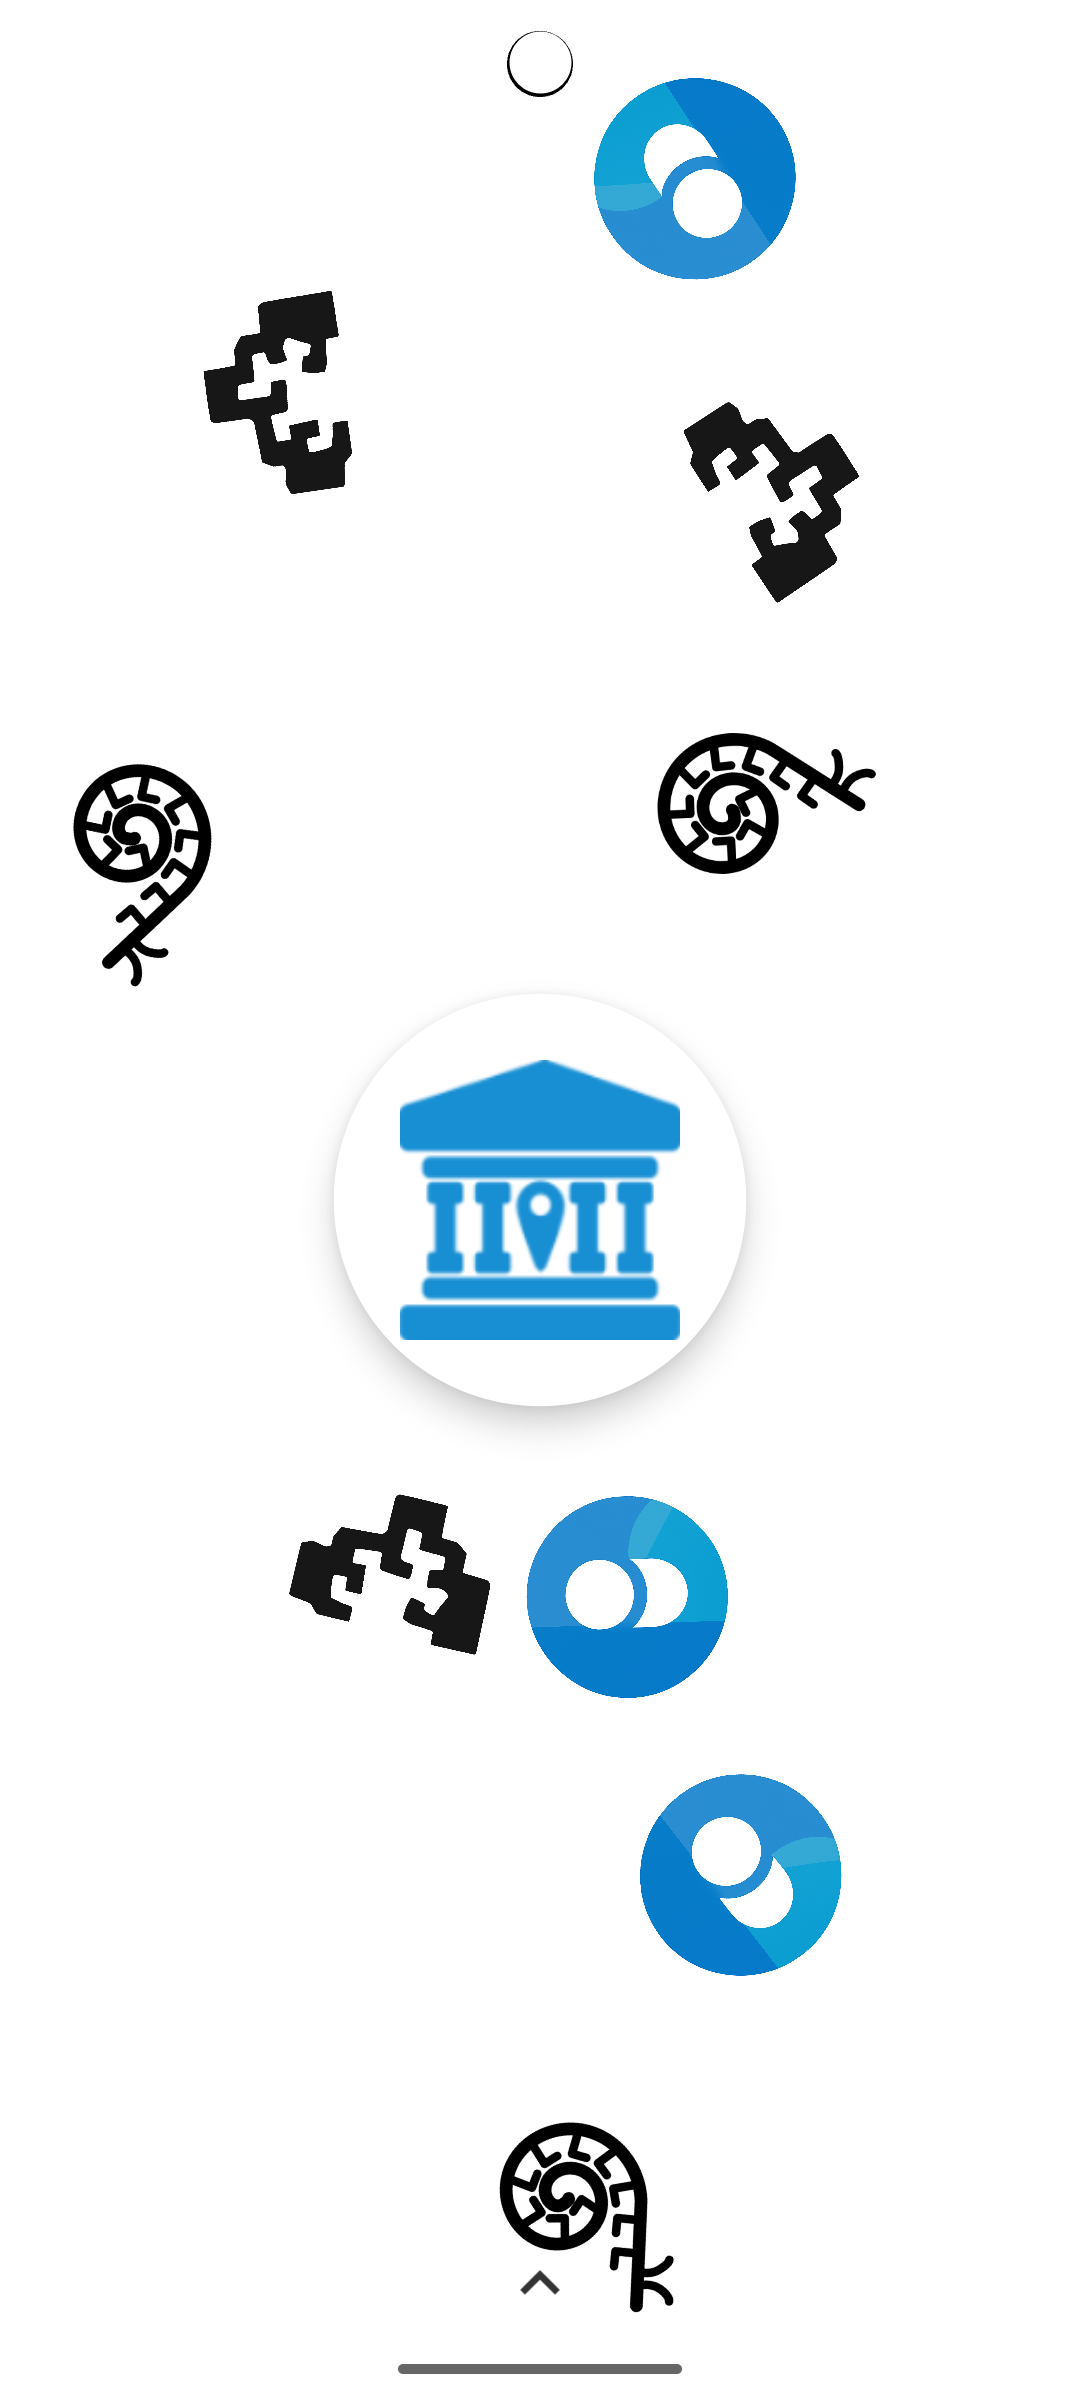
\includegraphics[scale=0.15]{../.img/splash.png}}
  \caption{\textit{Splash screen} inicial.}
  \label{fig:splash}
\end{figure}

\begin{figure}[htbp]
  \centering
  \subfigure[inicio de sesión]{\fbox{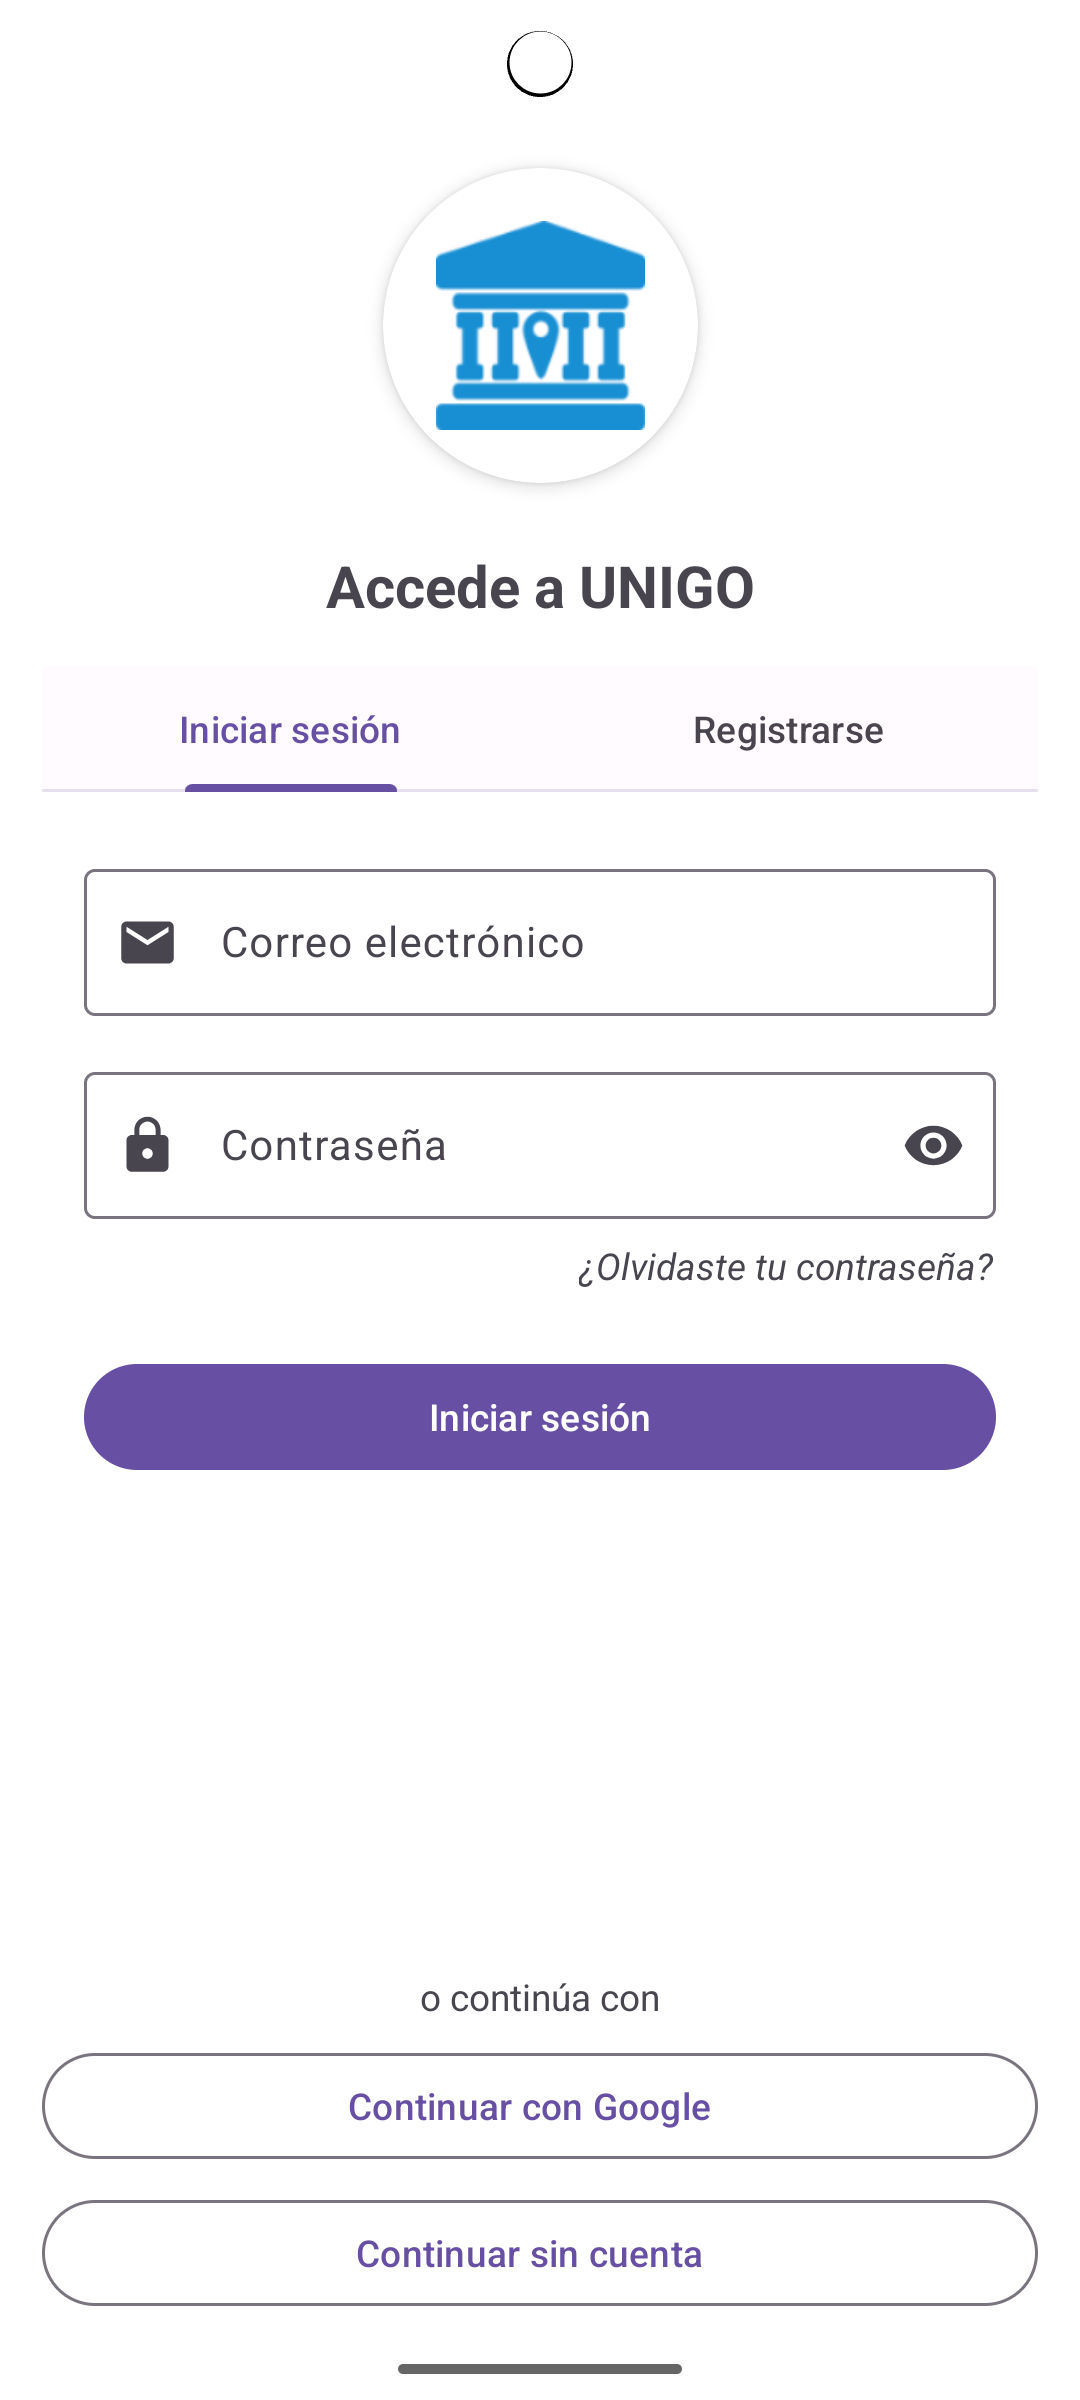
\includegraphics[scale=0.11]{../.img/inicio_sesion.png}}}
  \hspace{0.5cm}
  \subfigure[registro]{\fbox{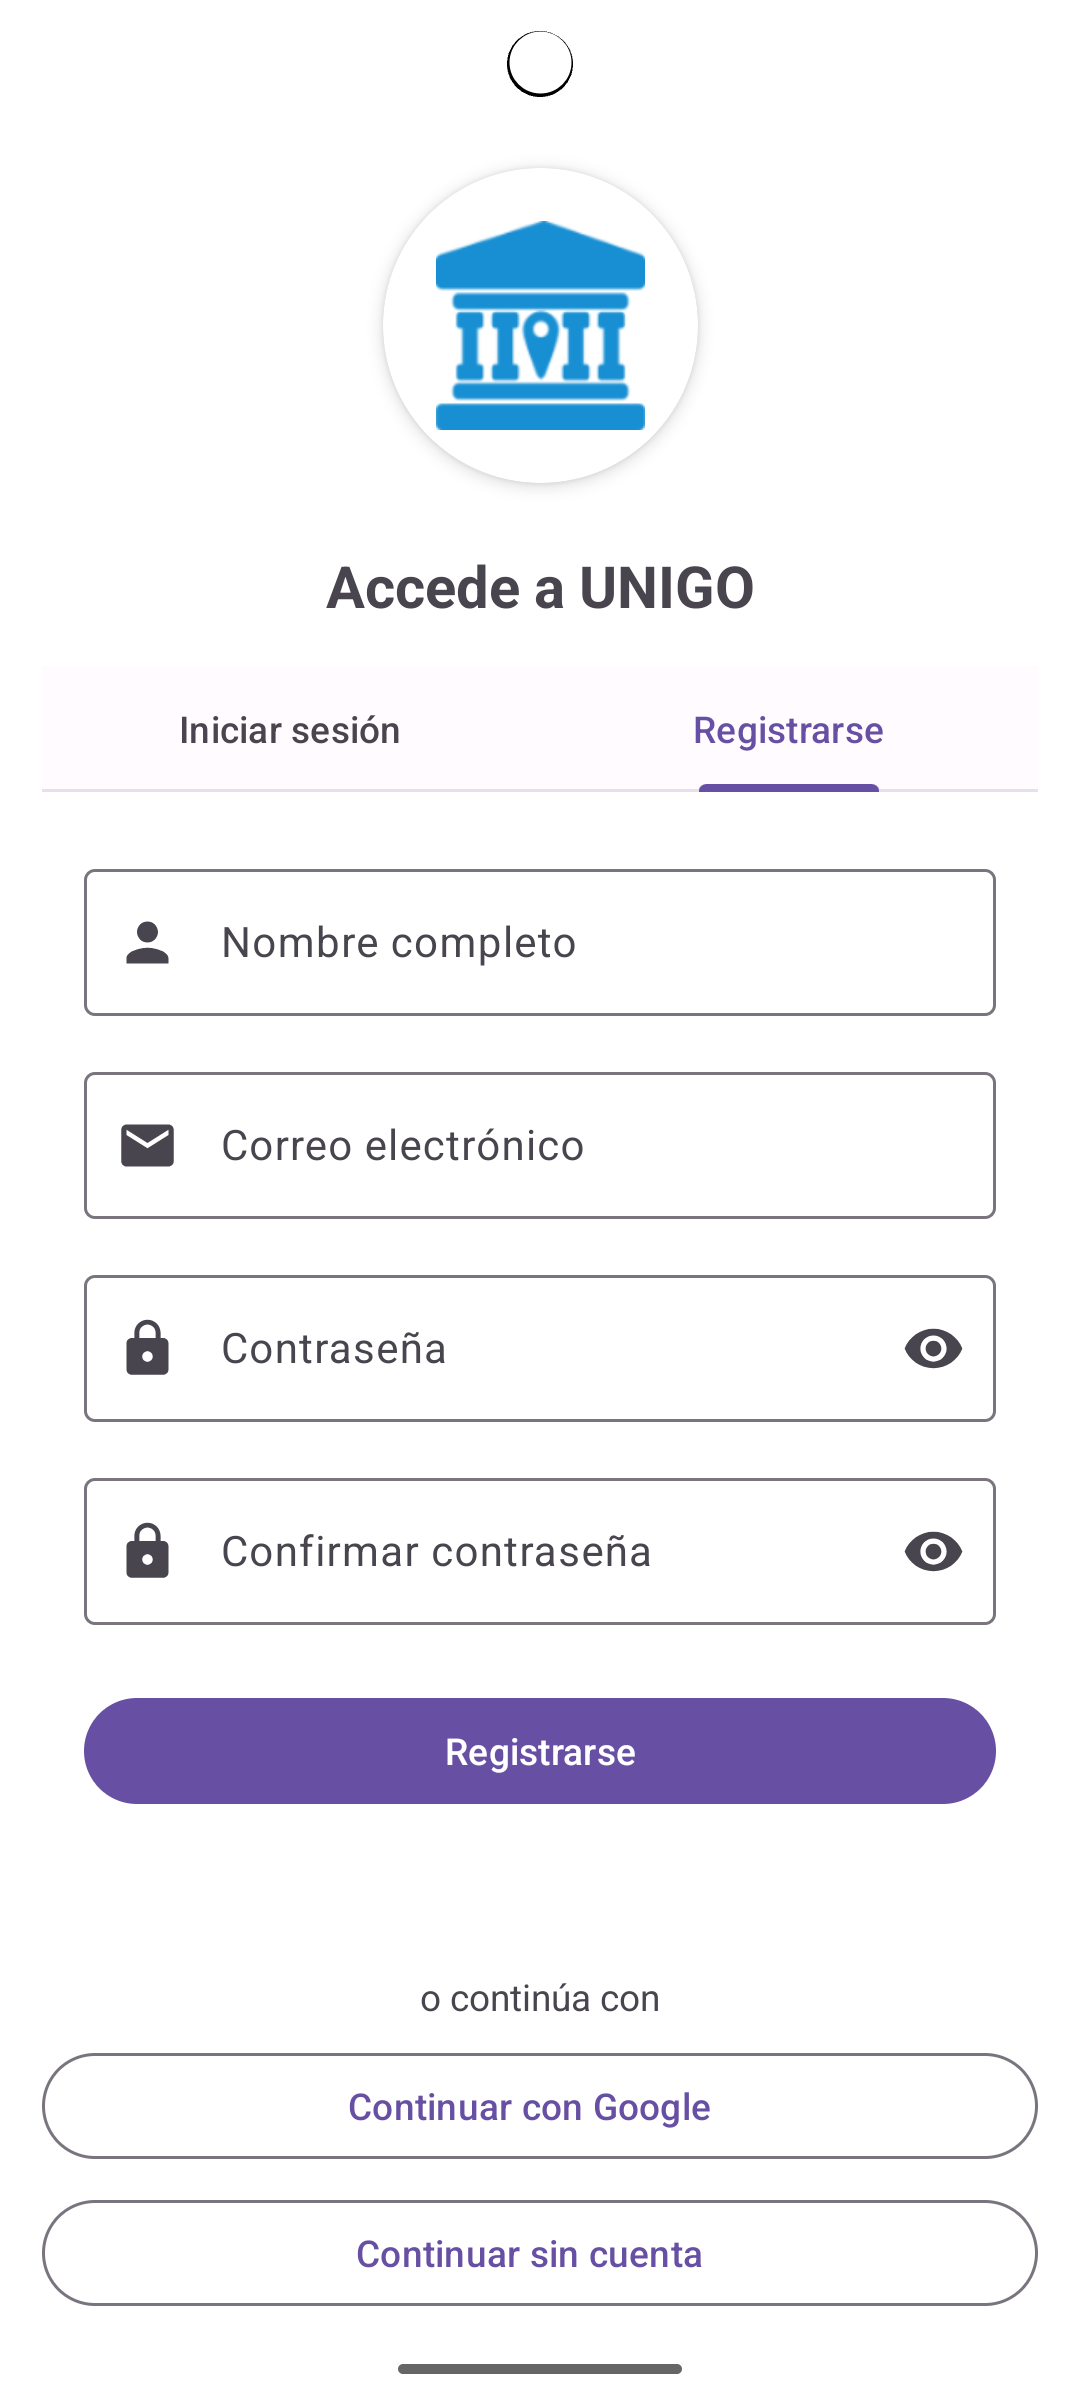
\includegraphics[scale=0.11]{../.img/registro.png}}}
  \caption{Pantallas de inicio de sesión.}
  \label{fig:inicial}
\end{figure}

\section{Mapa}
  Una vez iniciada la sesión, la aplicación solicitará permisos para acceder a nuestra ubicación. Al concederlos, se mostrará un mapa con varios iconos que indican tanto nuestra posición como la del campus universitario (Figura \ref{fig:map_default}). Mediante los botones disponibles, podremos seleccionar el medio de transporte y el centro al que deseamos dirigirnos (Figura \ref{fig:map_select}).

  Con un medio de transporte y un centro seleccionados, al pulsar sobre el botón en la parte inferior izquierda de la pantalla, se mostrará la ruta desde la posición del usuario al destino.
  
  En el caso de los autobuses, se marcará la línea entera que corresponde al trayecto. Se mostrará el camino que tiene que seguir el usuario, andando, para llegar a la parada más cercana de la línea. Además, pulsando sobre esa parada, aparecerá información sobre los horarios de la línea. También se marcará la ruta desde la parada en la que tiene que bajarse el usuario hasta el destino.

  

% mapa
\begin{figure}[htbp]
  \centering
  \fbox{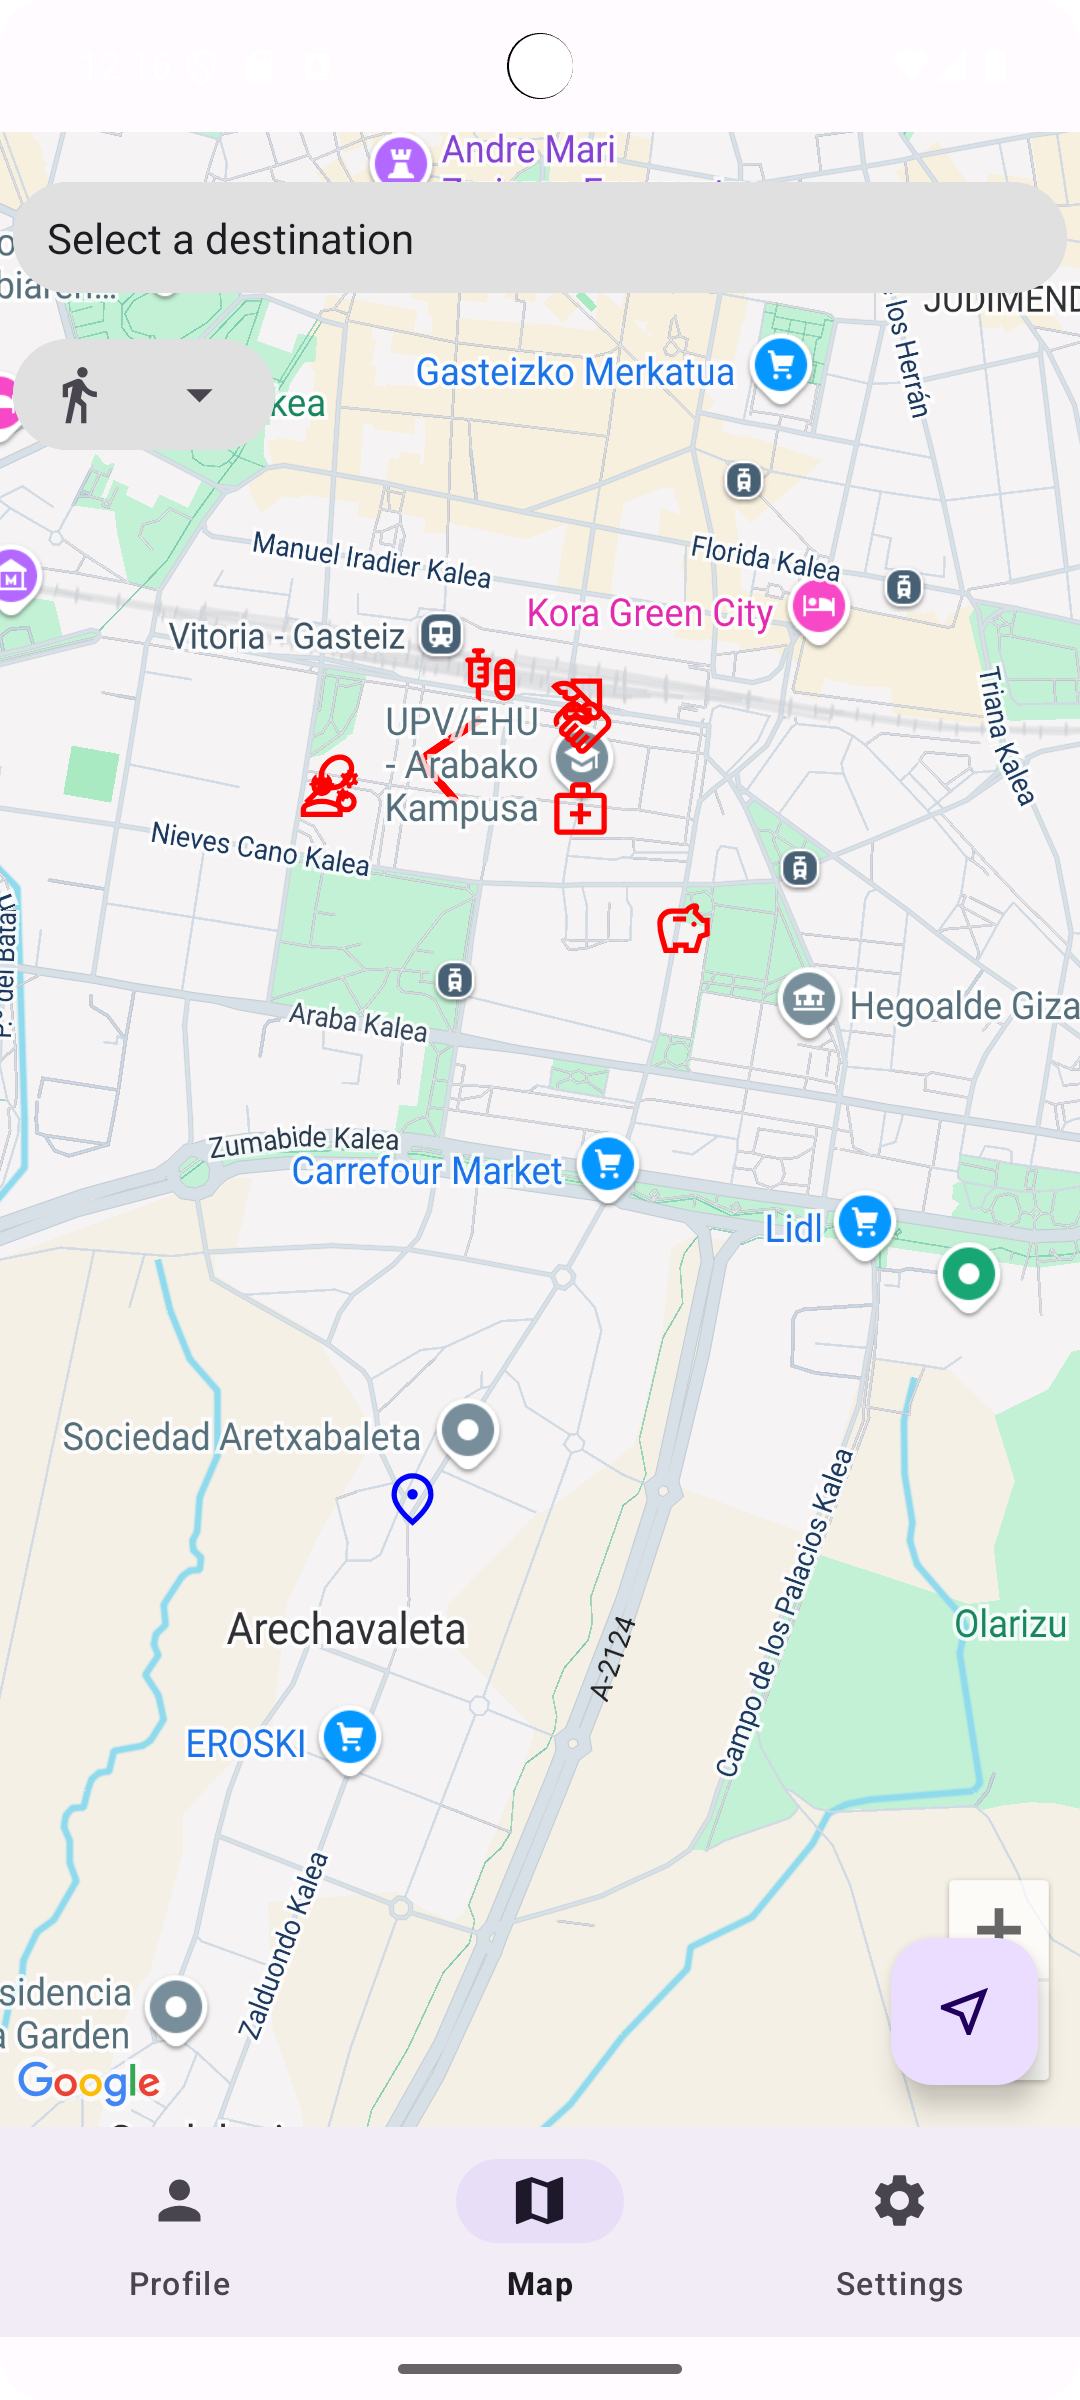
\includegraphics[scale=0.15]{../.img/map_default.png}}
  \caption{\textit{Map screen} inical.}
  \label{fig:map_default}
\end{figure}

\begin{figure}[htbp]
  \centering
  \subfigure[seleccionar destino]{\fbox{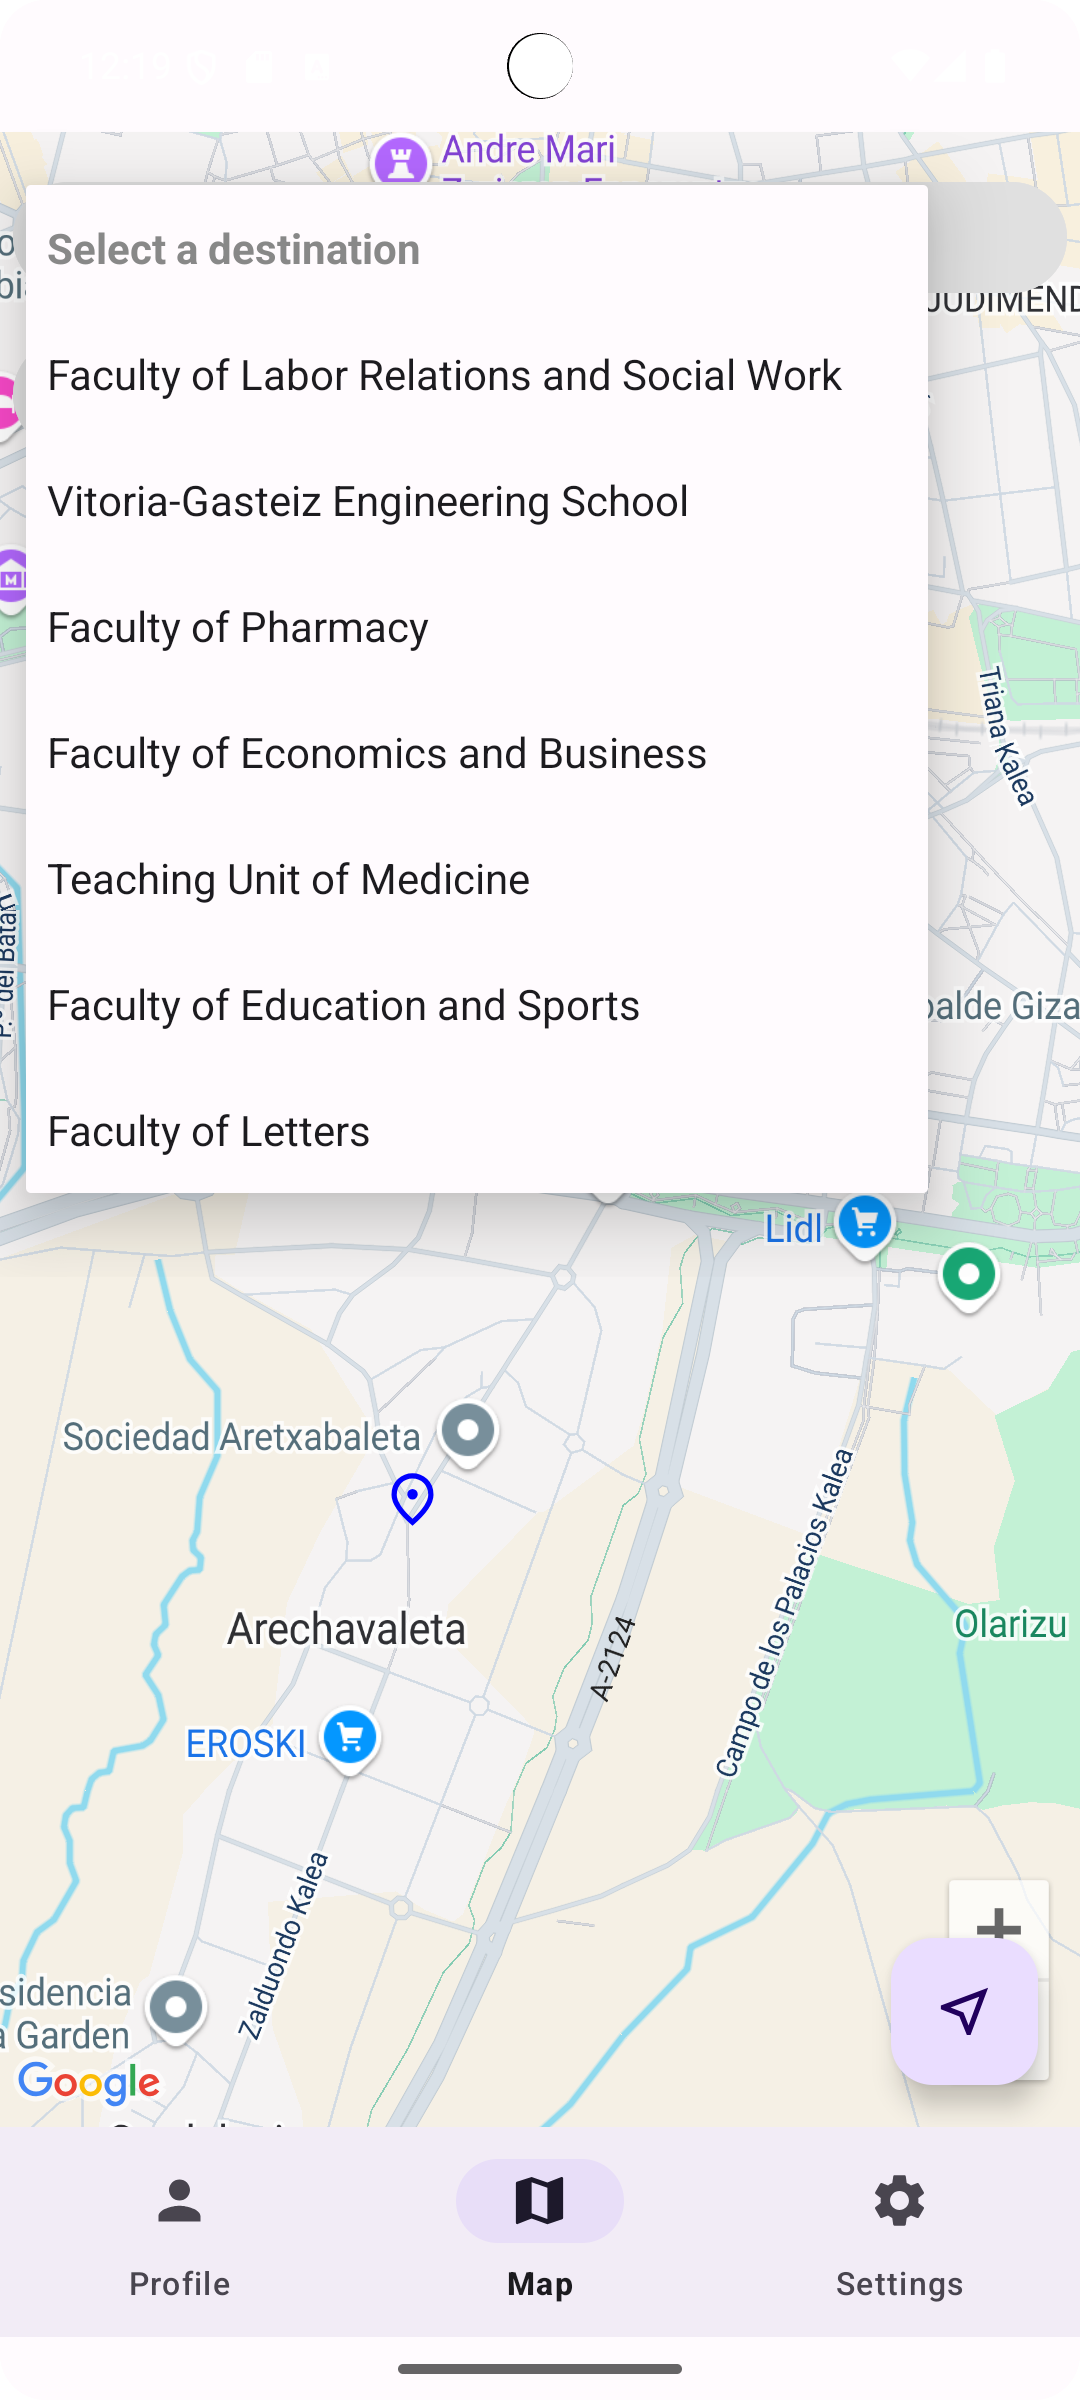
\includegraphics[scale=0.11]{../.img/map_select_dest.png}}}
  \hspace{0.5cm}
  \subfigure[seleccionar medio de transporte]{\fbox{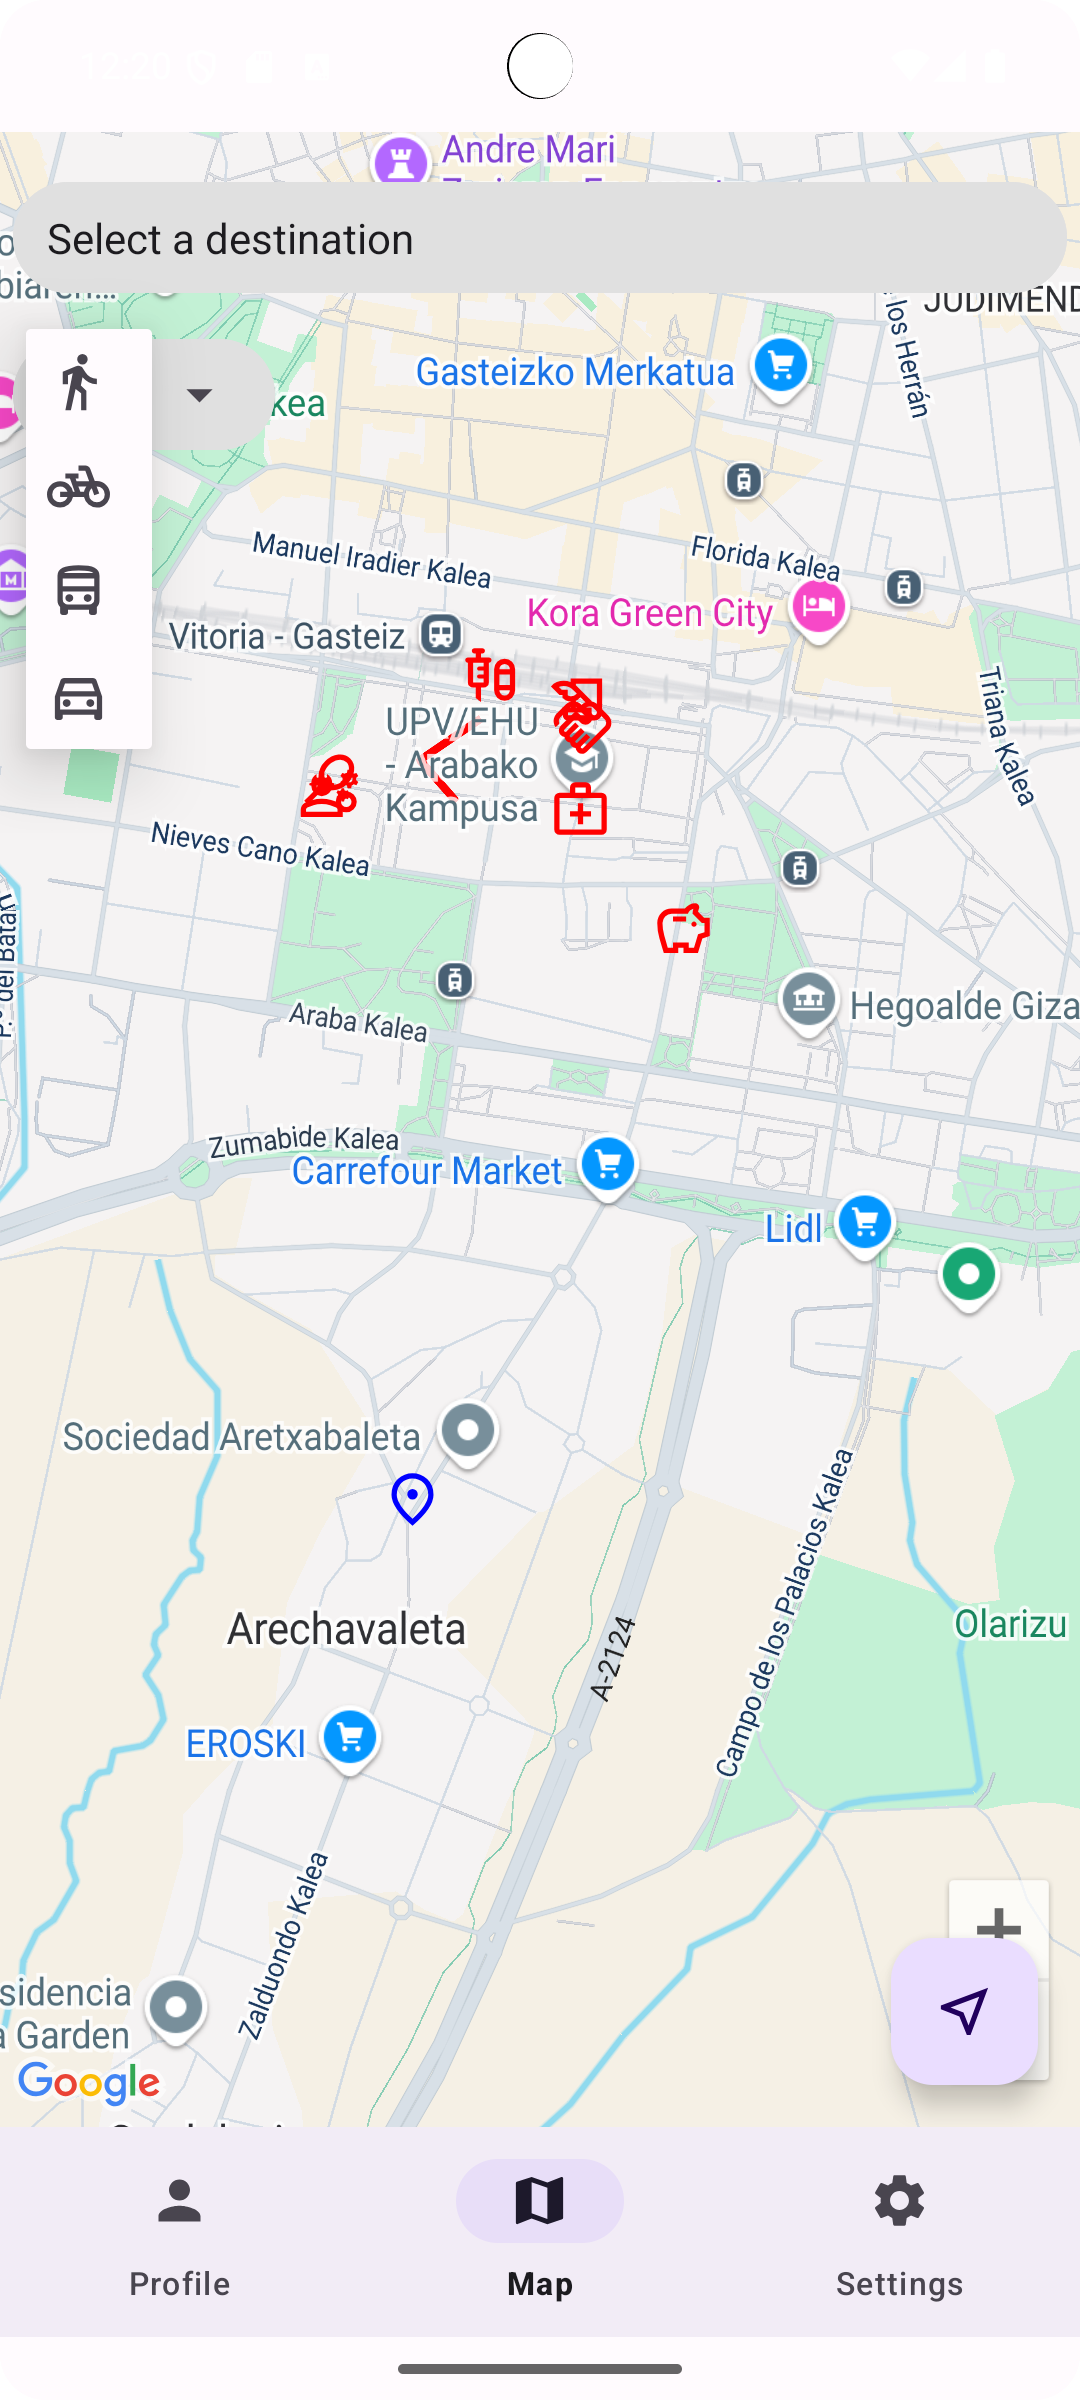
\includegraphics[scale=0.11]{../.img/map_select_transport.png}}}
  \caption{\textit{Map screen} opciones.}
  \label{fig:map_select}
\end{figure}

% TODO: poner una busqueda todo chula + Texto texto

\section{Perfil}
  En el fragmento de perfil, se mostrará el nombre completo del usuario, el correo electrónico y la foto de perfil. Si se ha iniciado sesión mediante usuario y contraseña, toda esa información se podrá editar. Asimismo, habrá una opción para restablecer la contraseña. Si se ha iniciado sesión con Google, se podrá cambiar el nombre. En una sesión sin cuenta, solamente figurará 'Usuario anónimo', y no se podrá editar.

\begin{figure}[htbp]
  \centering
  \subfigure[usuario y contraseña]{\fbox{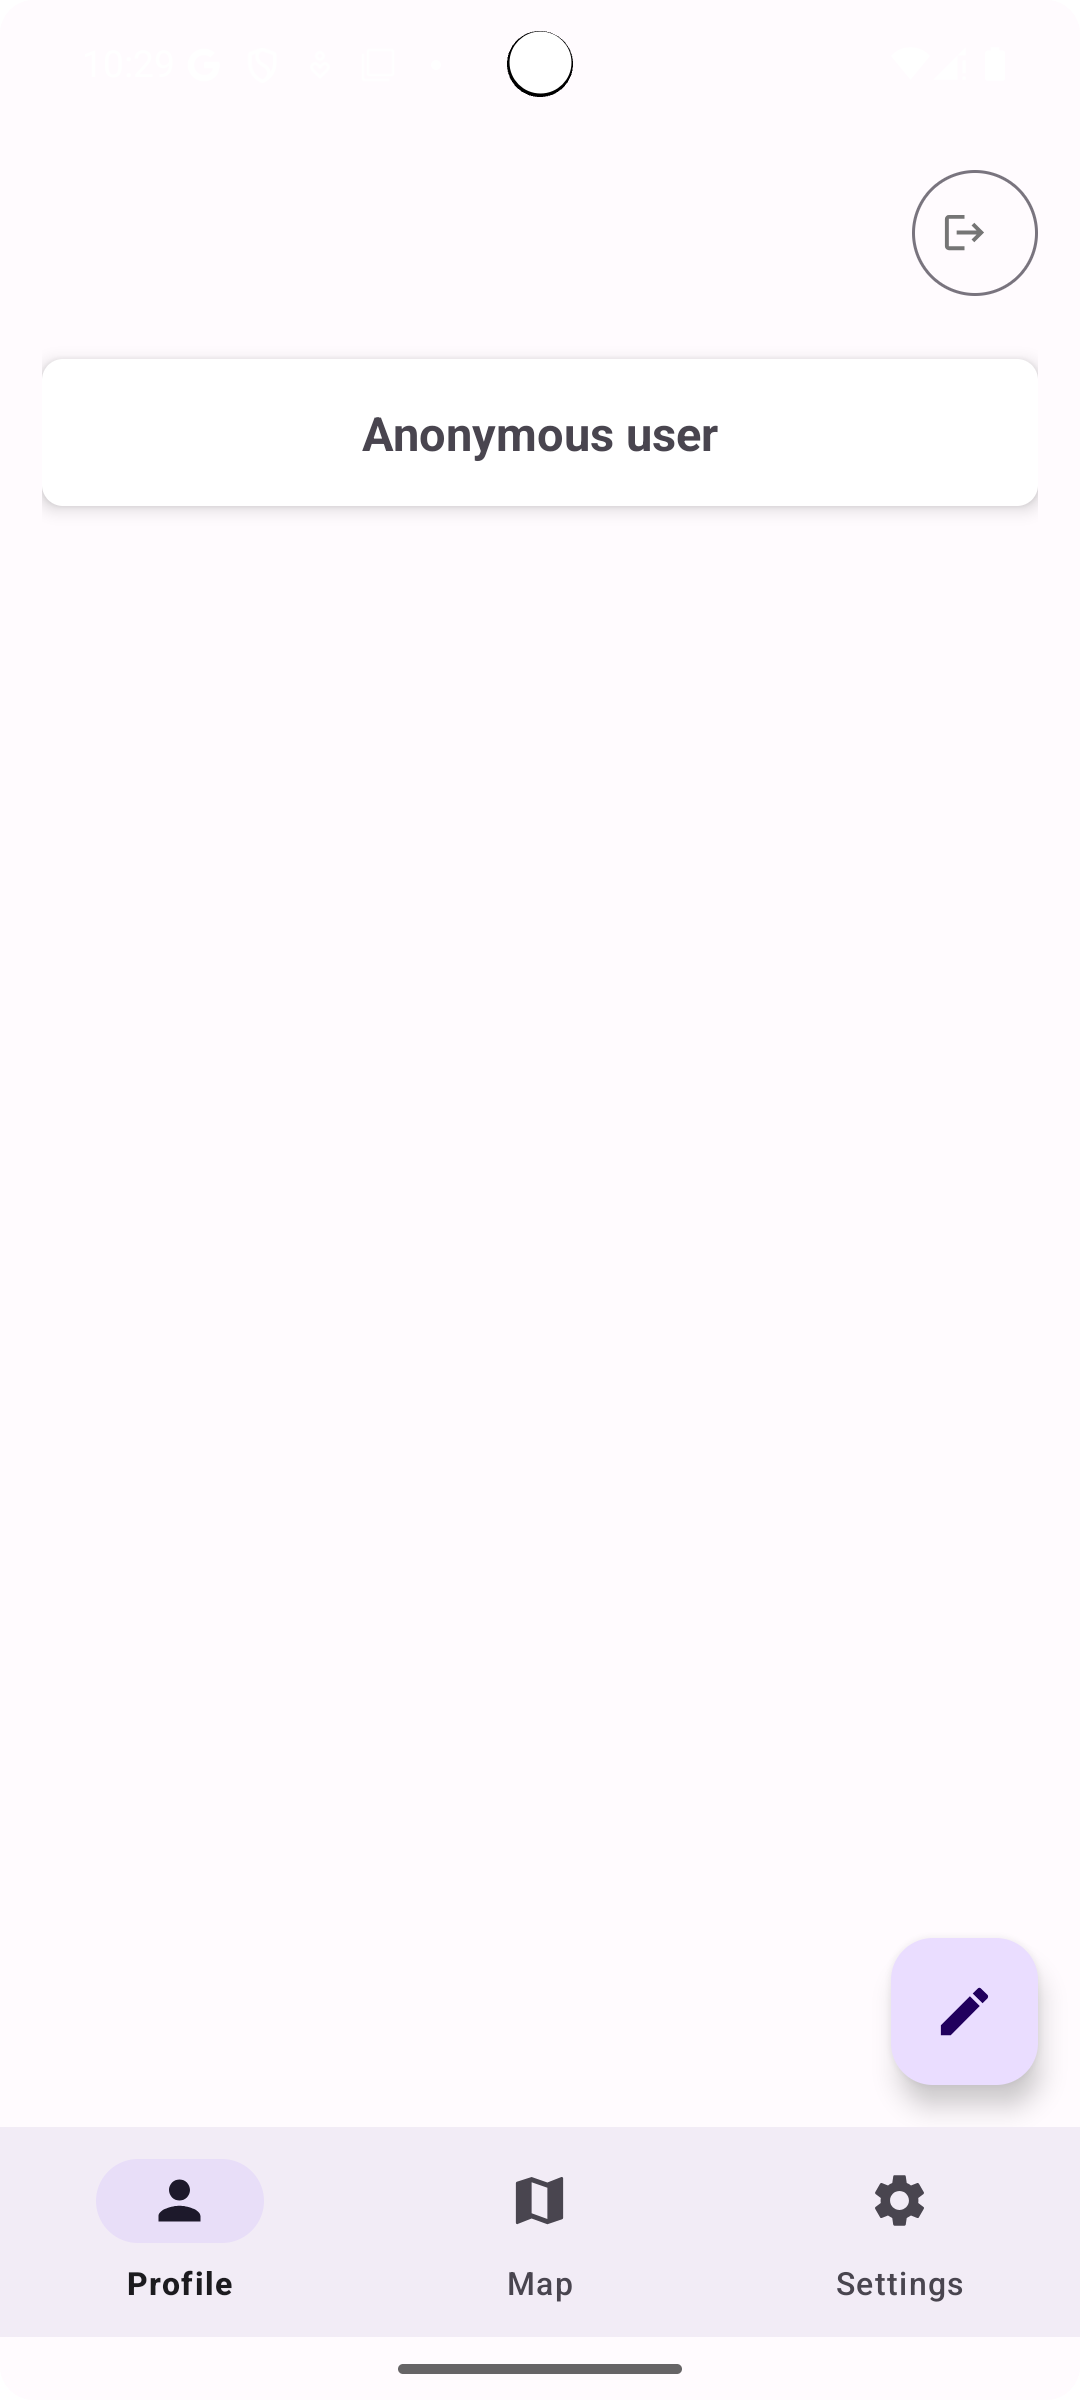
\includegraphics[scale=0.11]{../.img/perfil_anonimo.png}}}
  \hspace{0.5cm}
  \subfigure[sesión con Google]{\fbox{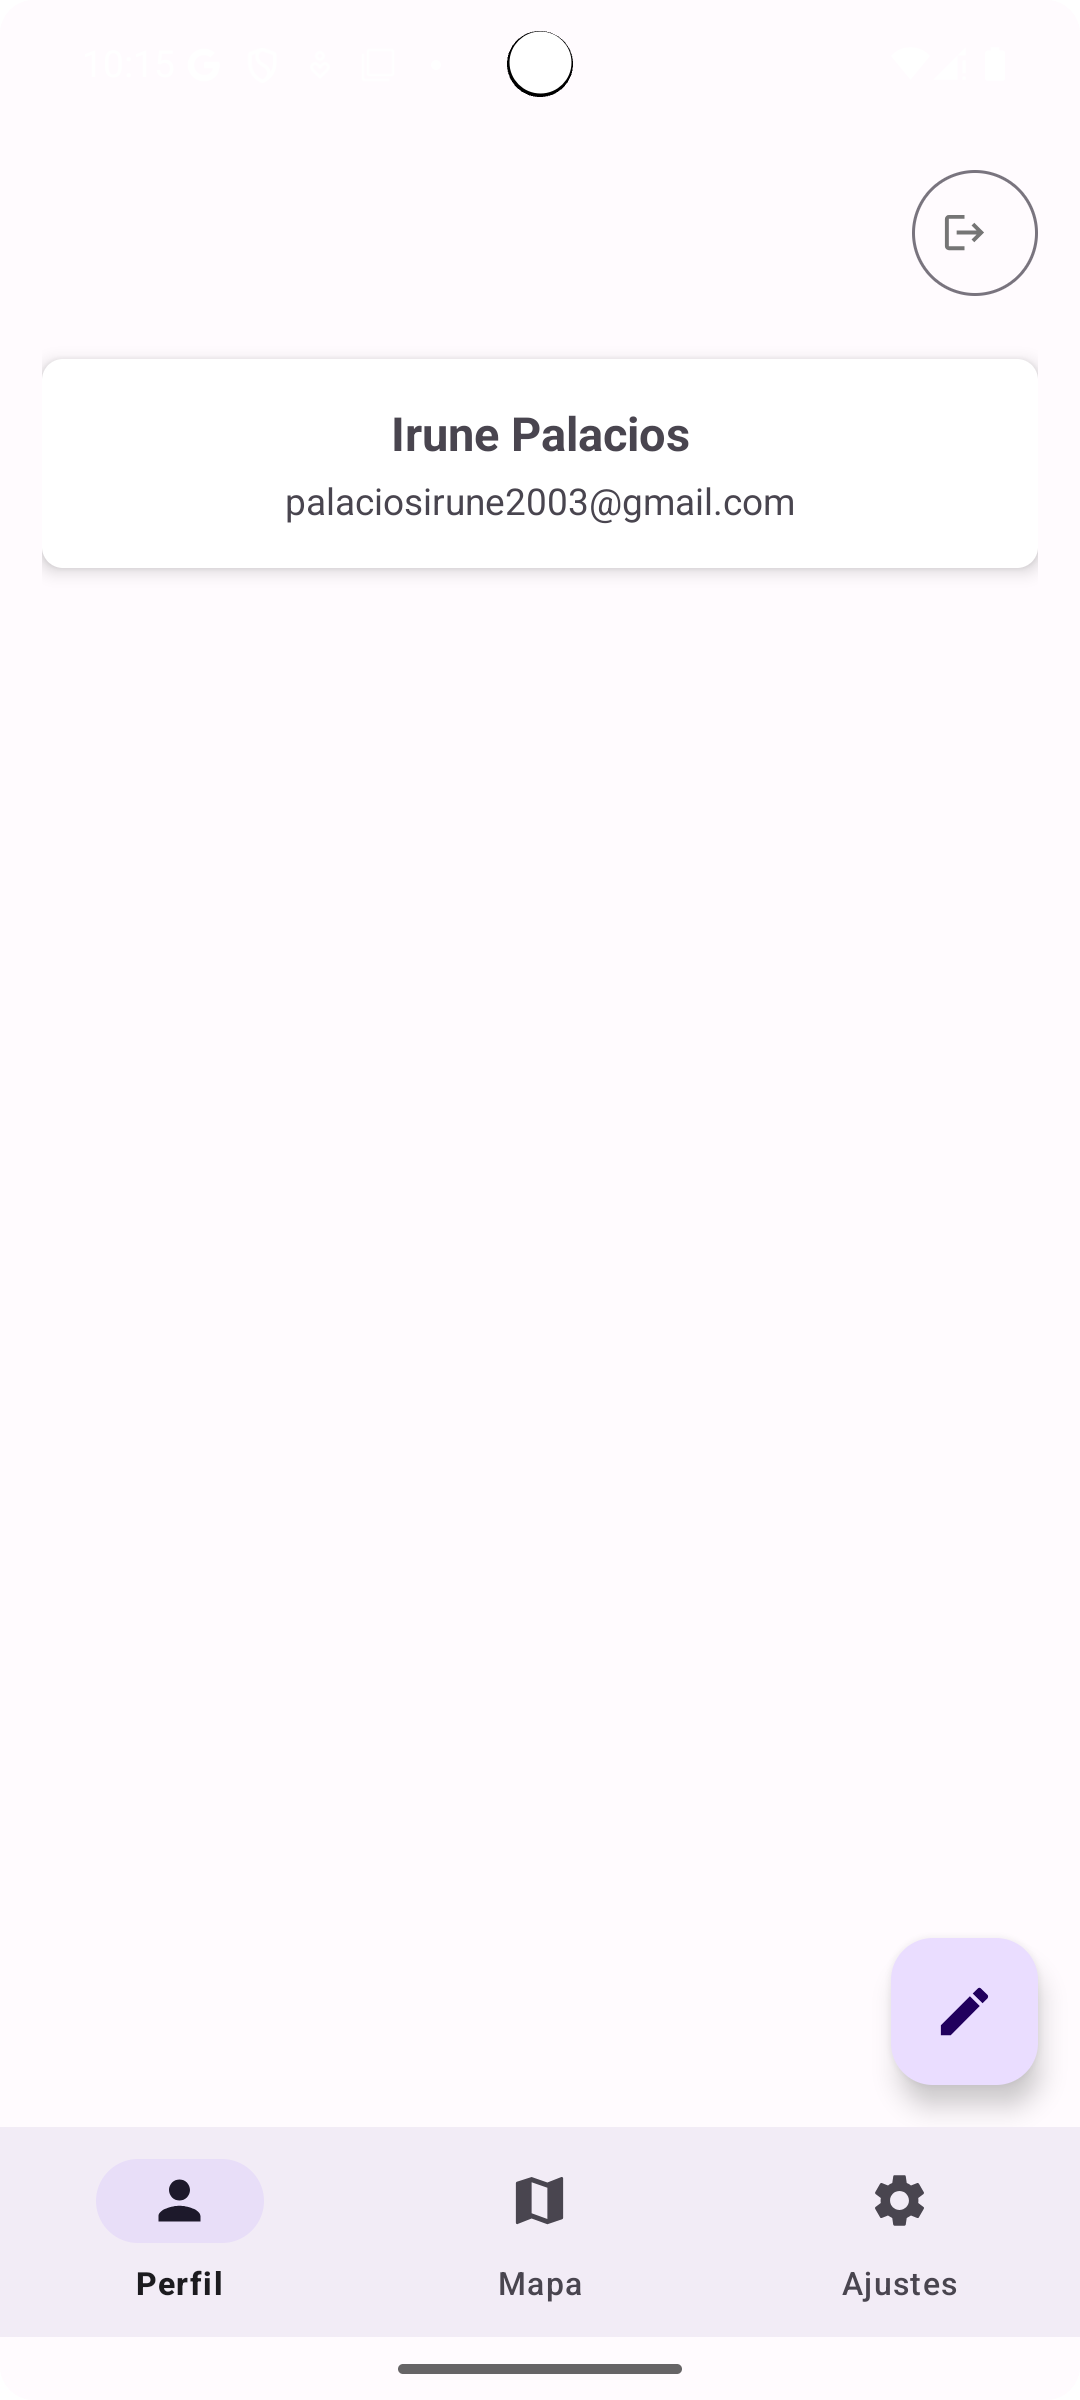
\includegraphics[scale=0.11]{../.img/perfil_google.png}}}
  \hspace{0.5cm}
  \subfigure[sesión anónima]{\fbox{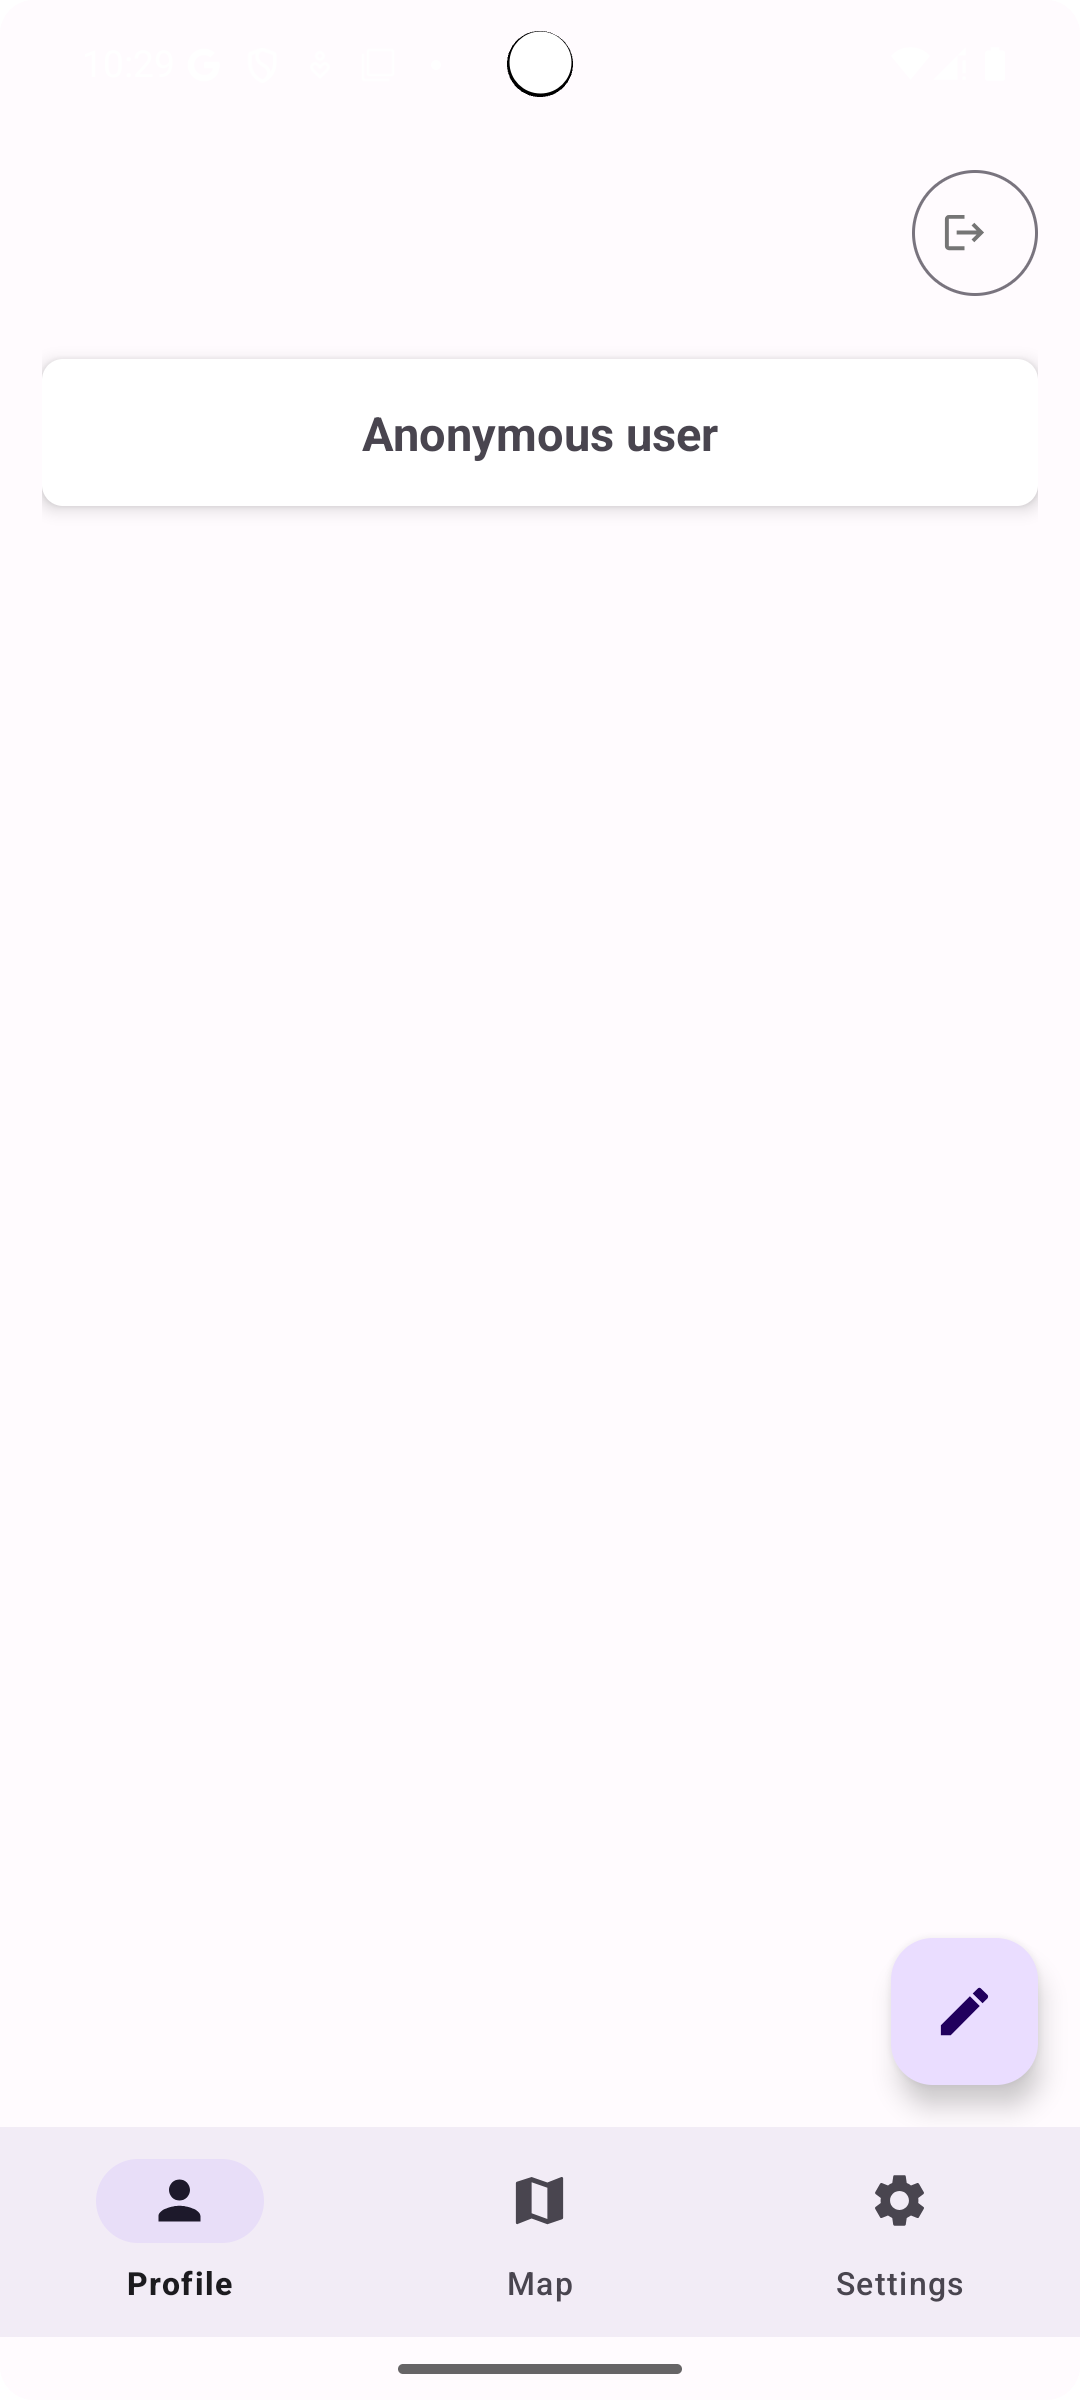
\includegraphics[scale=0.11]{../.img/perfil_anonimo.png}}}
  \caption{Pantallas de perfil.}
  \label{fig:perfil}
\end{figure}

\section{Ajustes}
  En el fragmento de ajustes, el usuario podrá cambiar el tema y el idioma de la aplicación (Figura \ref{fig:ajustes}). Para el tema tendrá tres opciones: claro, oscuro o modo del sistema. El modo del sistema aplica la configuración de tema del dispositivo. Para el idioma, podrá elegir entre castellano, euskera o inglés.

% ajustes
\begin{figure}[htbp]
  \centering
  \subfigure[tema claro]{\fbox{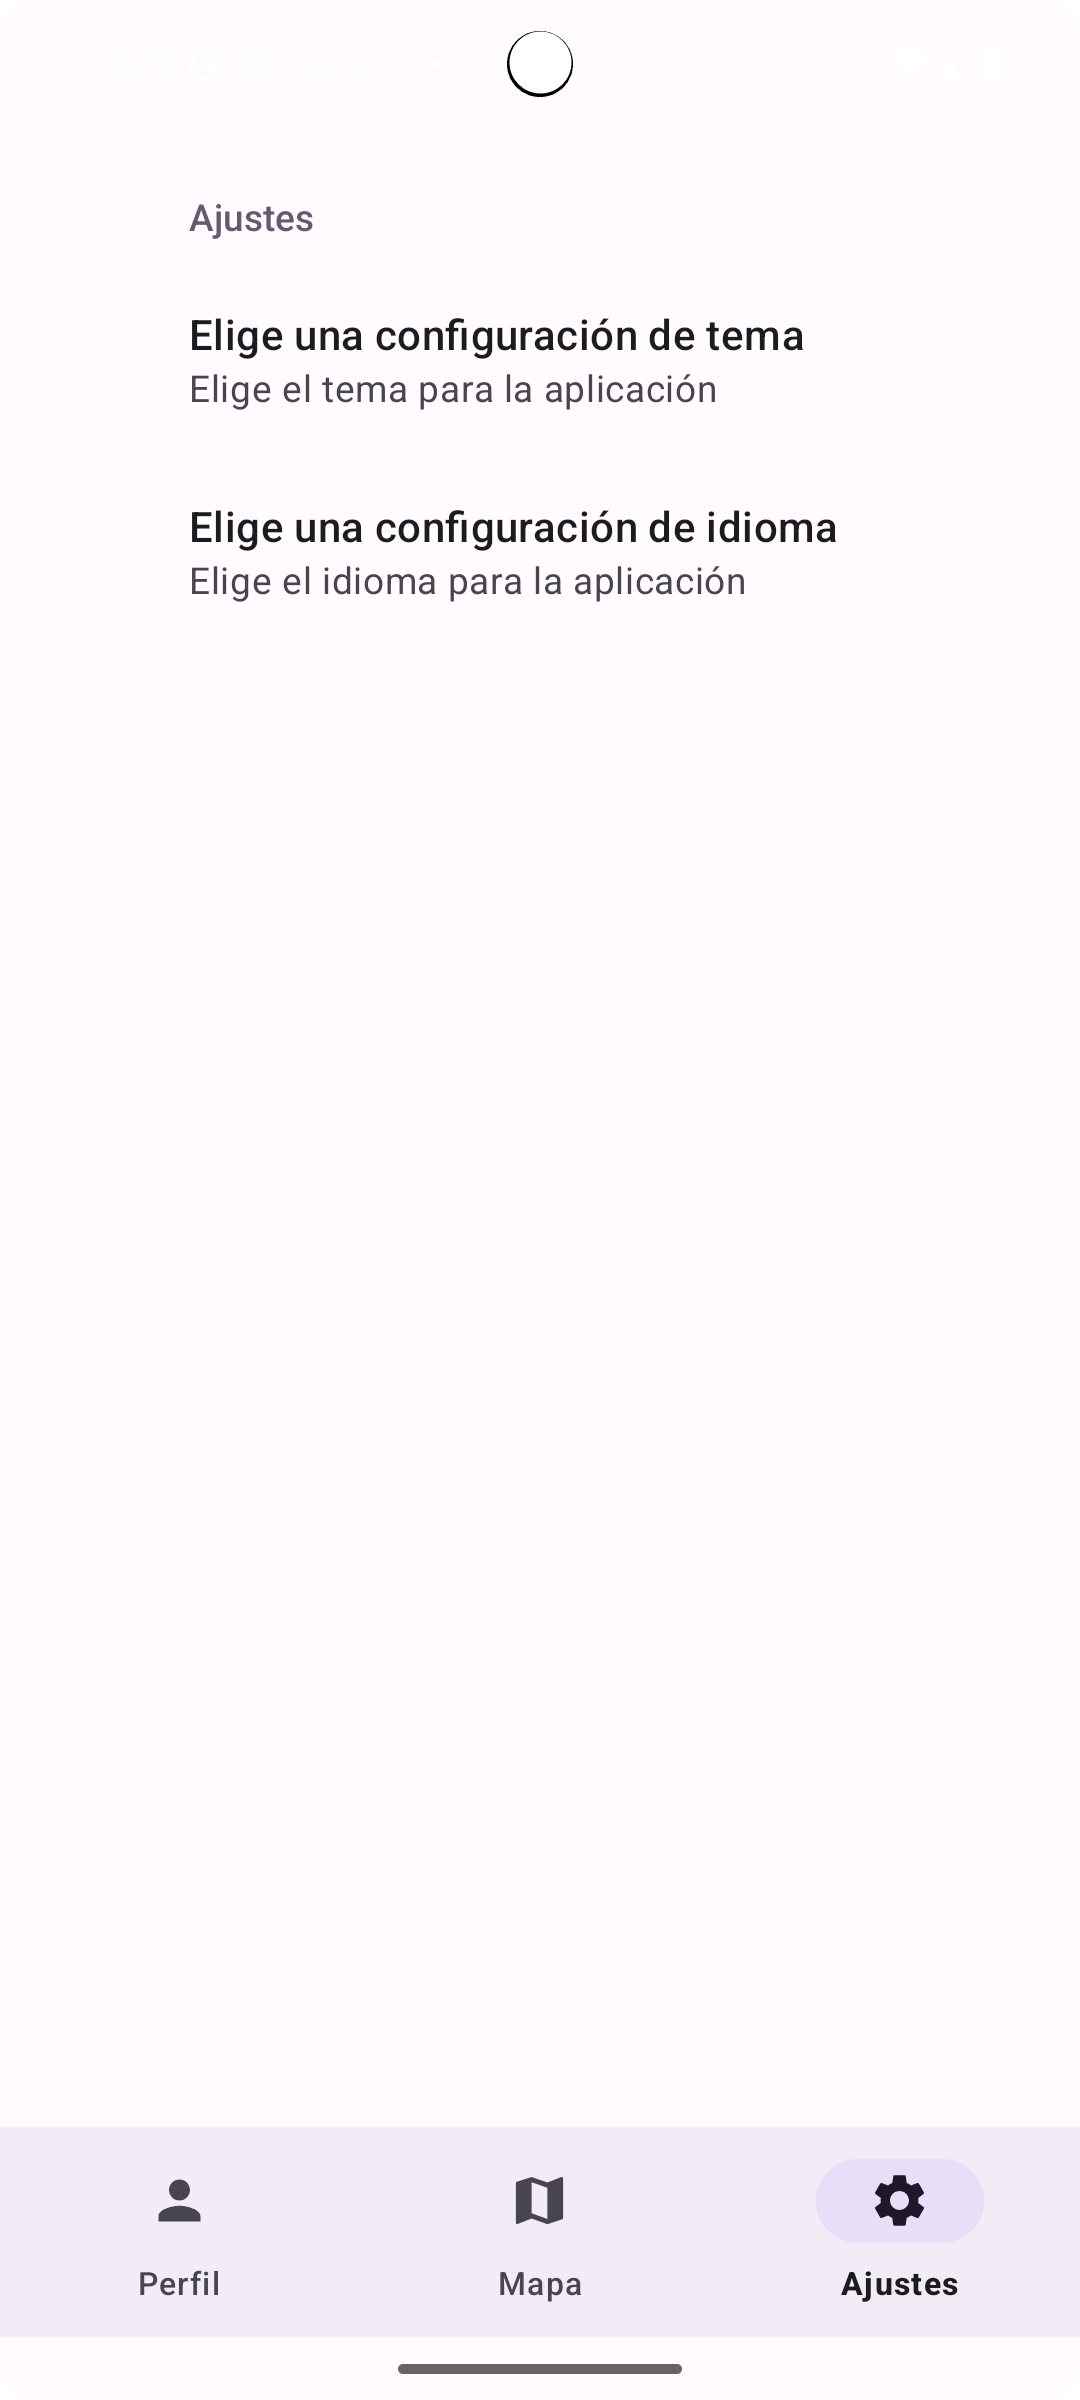
\includegraphics[scale=0.11]{../.img/ajustes_claro.png}}}
  \hspace{0.5cm}
  \subfigure[tema oscuro]{\fbox{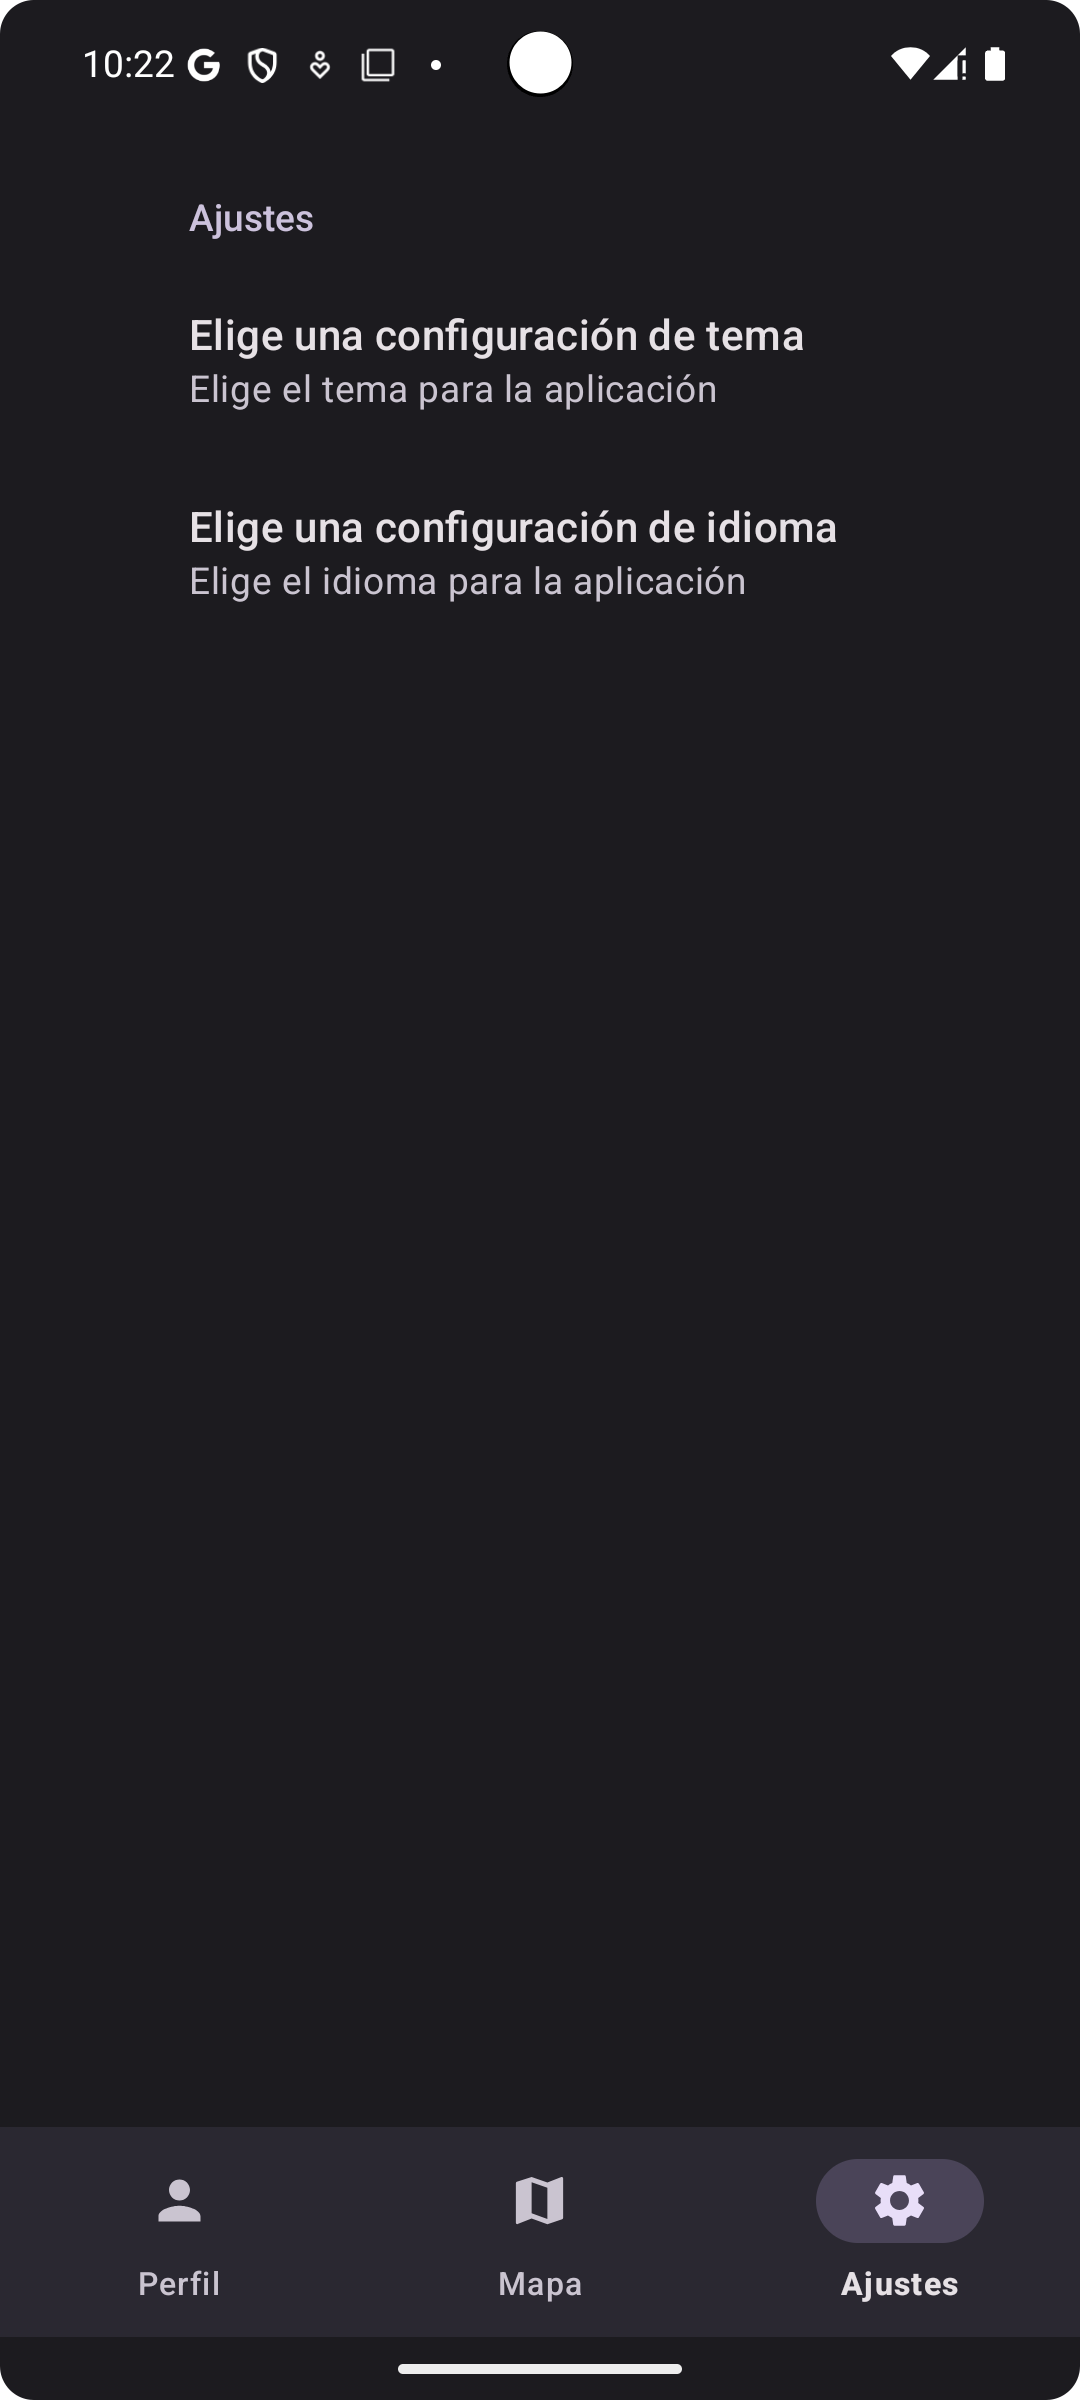
\includegraphics[scale=0.11]{../.img/ajustes_oscuro.png}}}
  \hspace{5cm}
  \subfigure[idioma en inglés]{\fbox{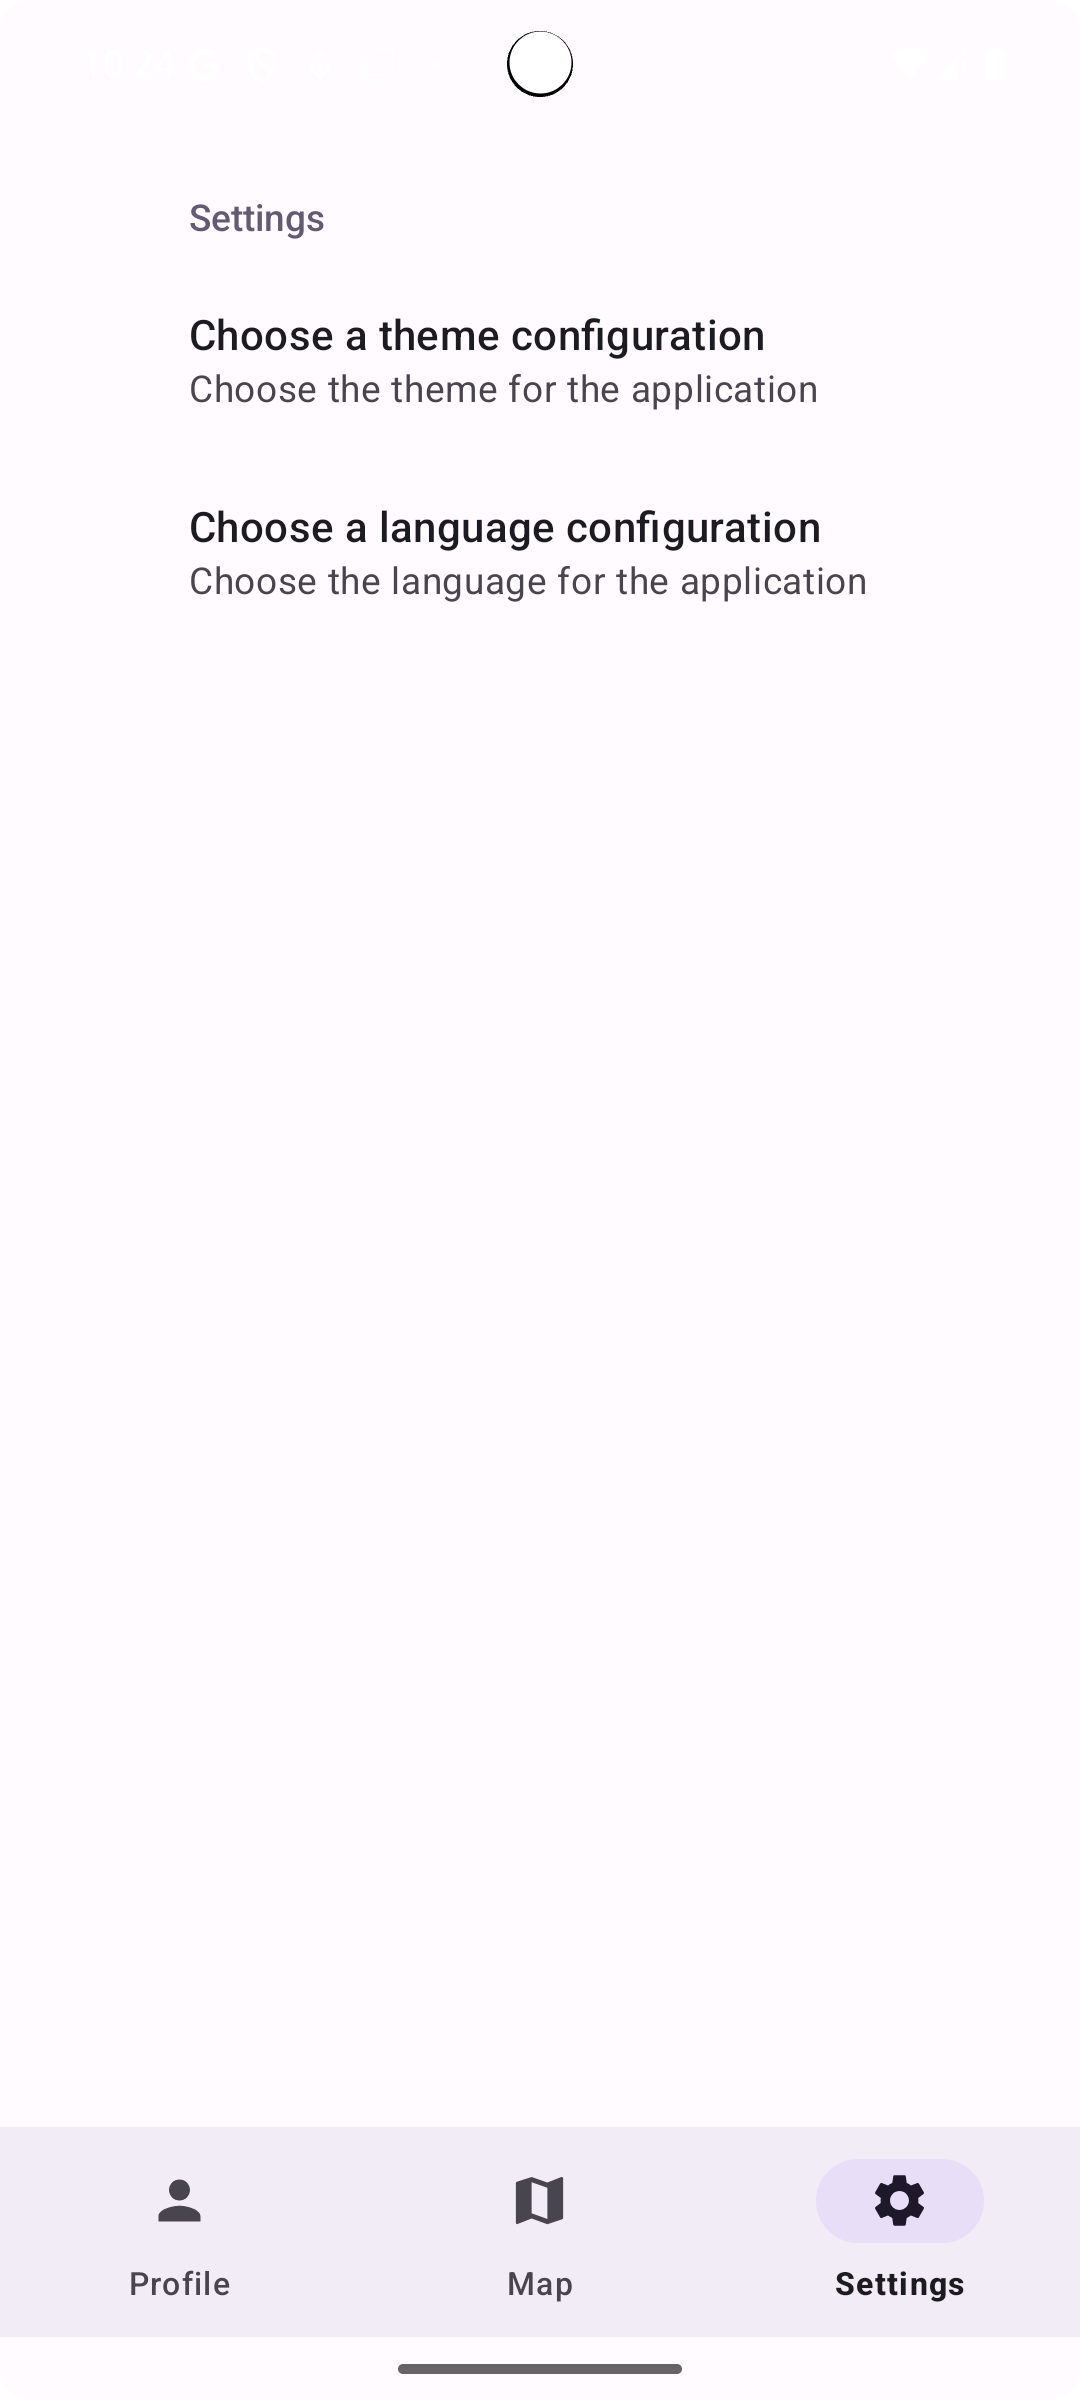
\includegraphics[scale=0.11]{../.img/ajustes_english.png}}}
  \hspace{0.5cm}
  \subfigure[idioma en euskera]{\fbox{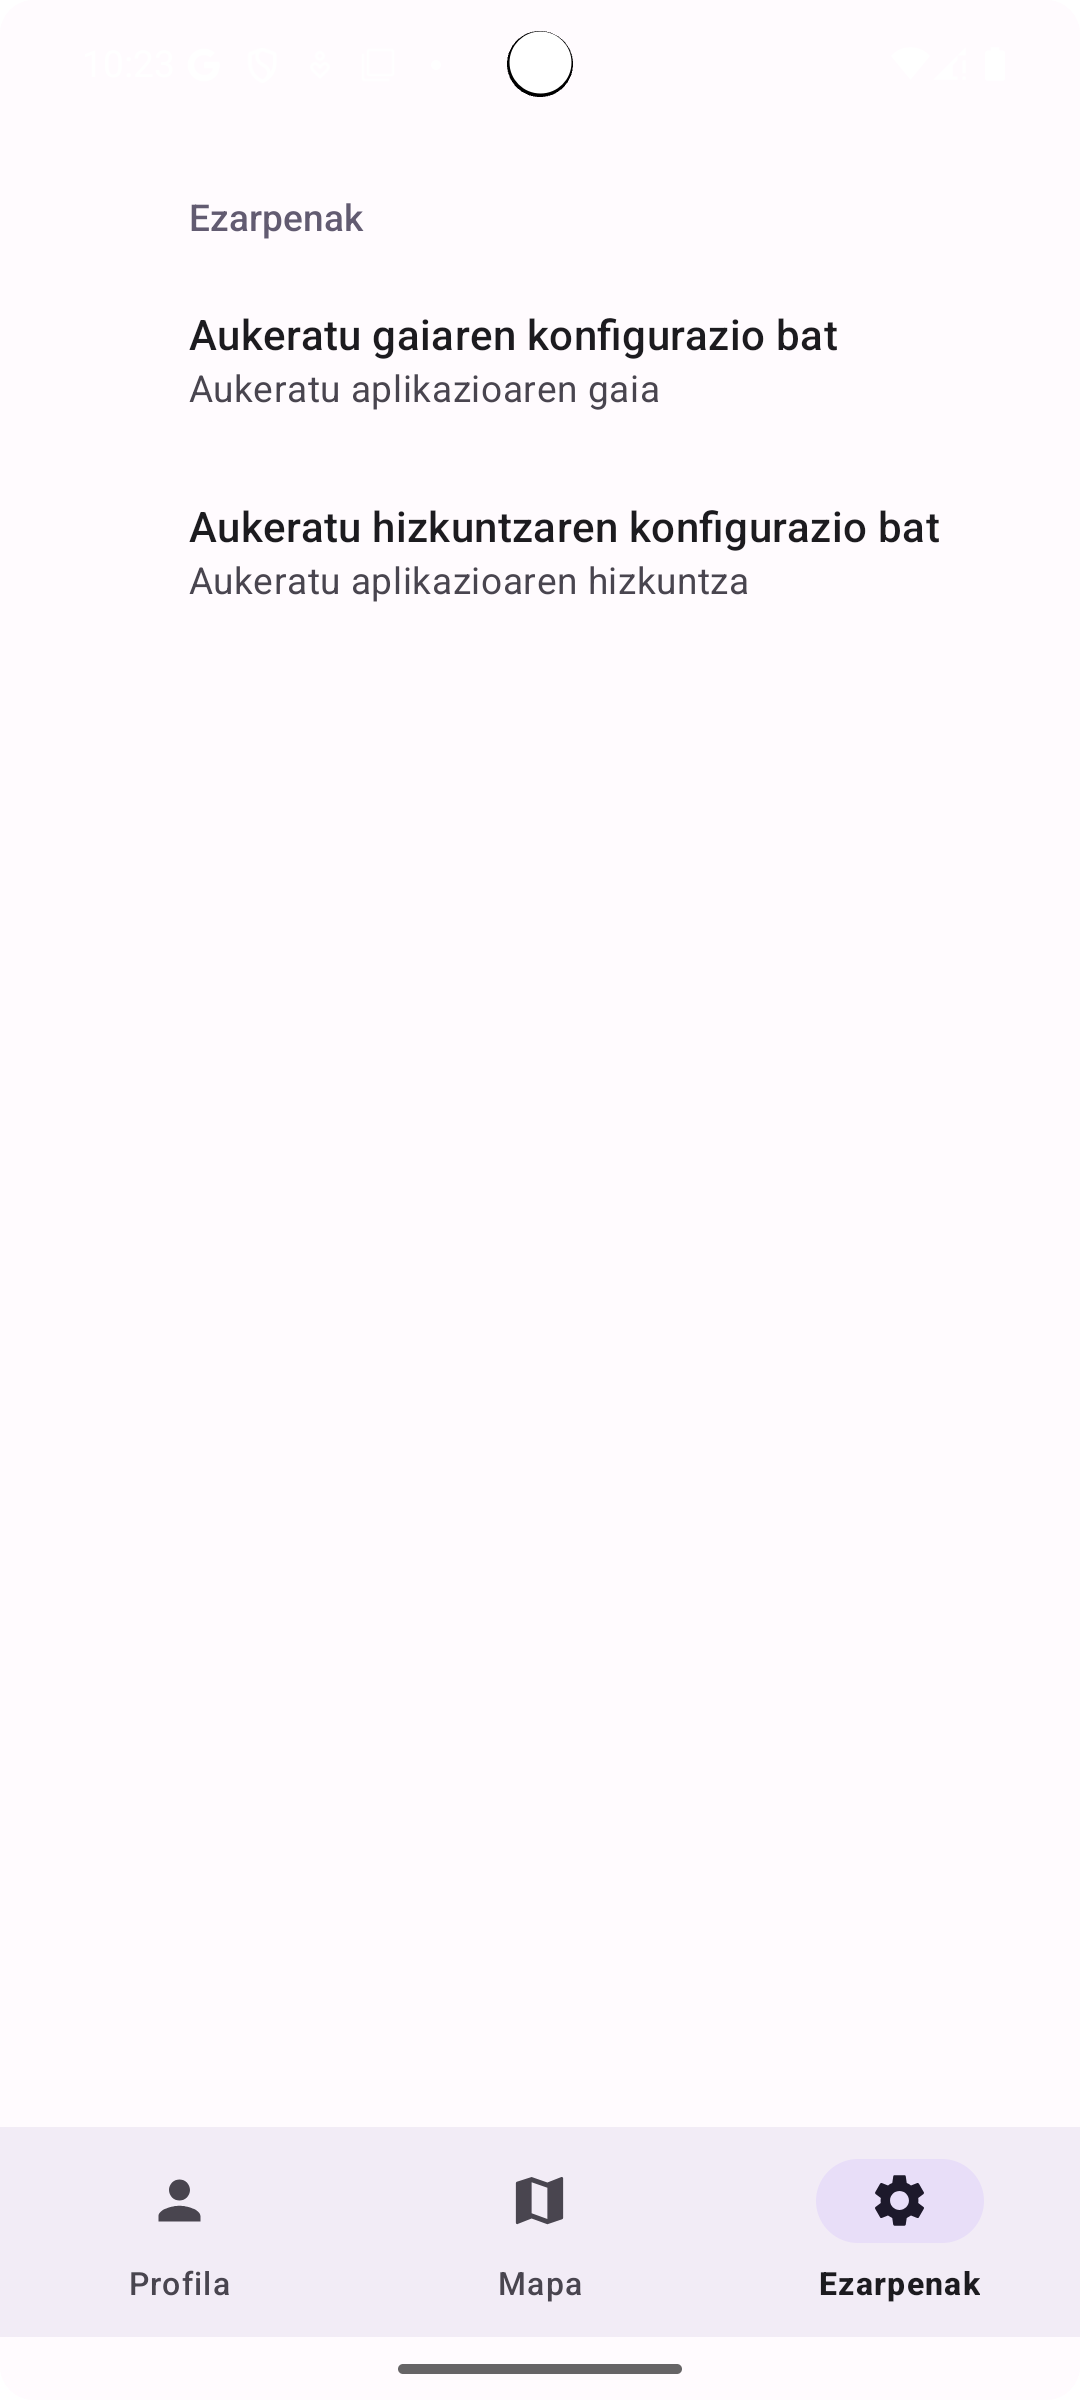
\includegraphics[scale=0.11]{../.img/ajustes_euskara.png}}}
  \caption{Pantalla de ajustes con distintas configuraciones.}
  \label{fig:ajustes}
\end{figure}

\end{document}
